\chapter{Related Work}
\label{chapter-related-work}
\begin{figure}
    \centering
    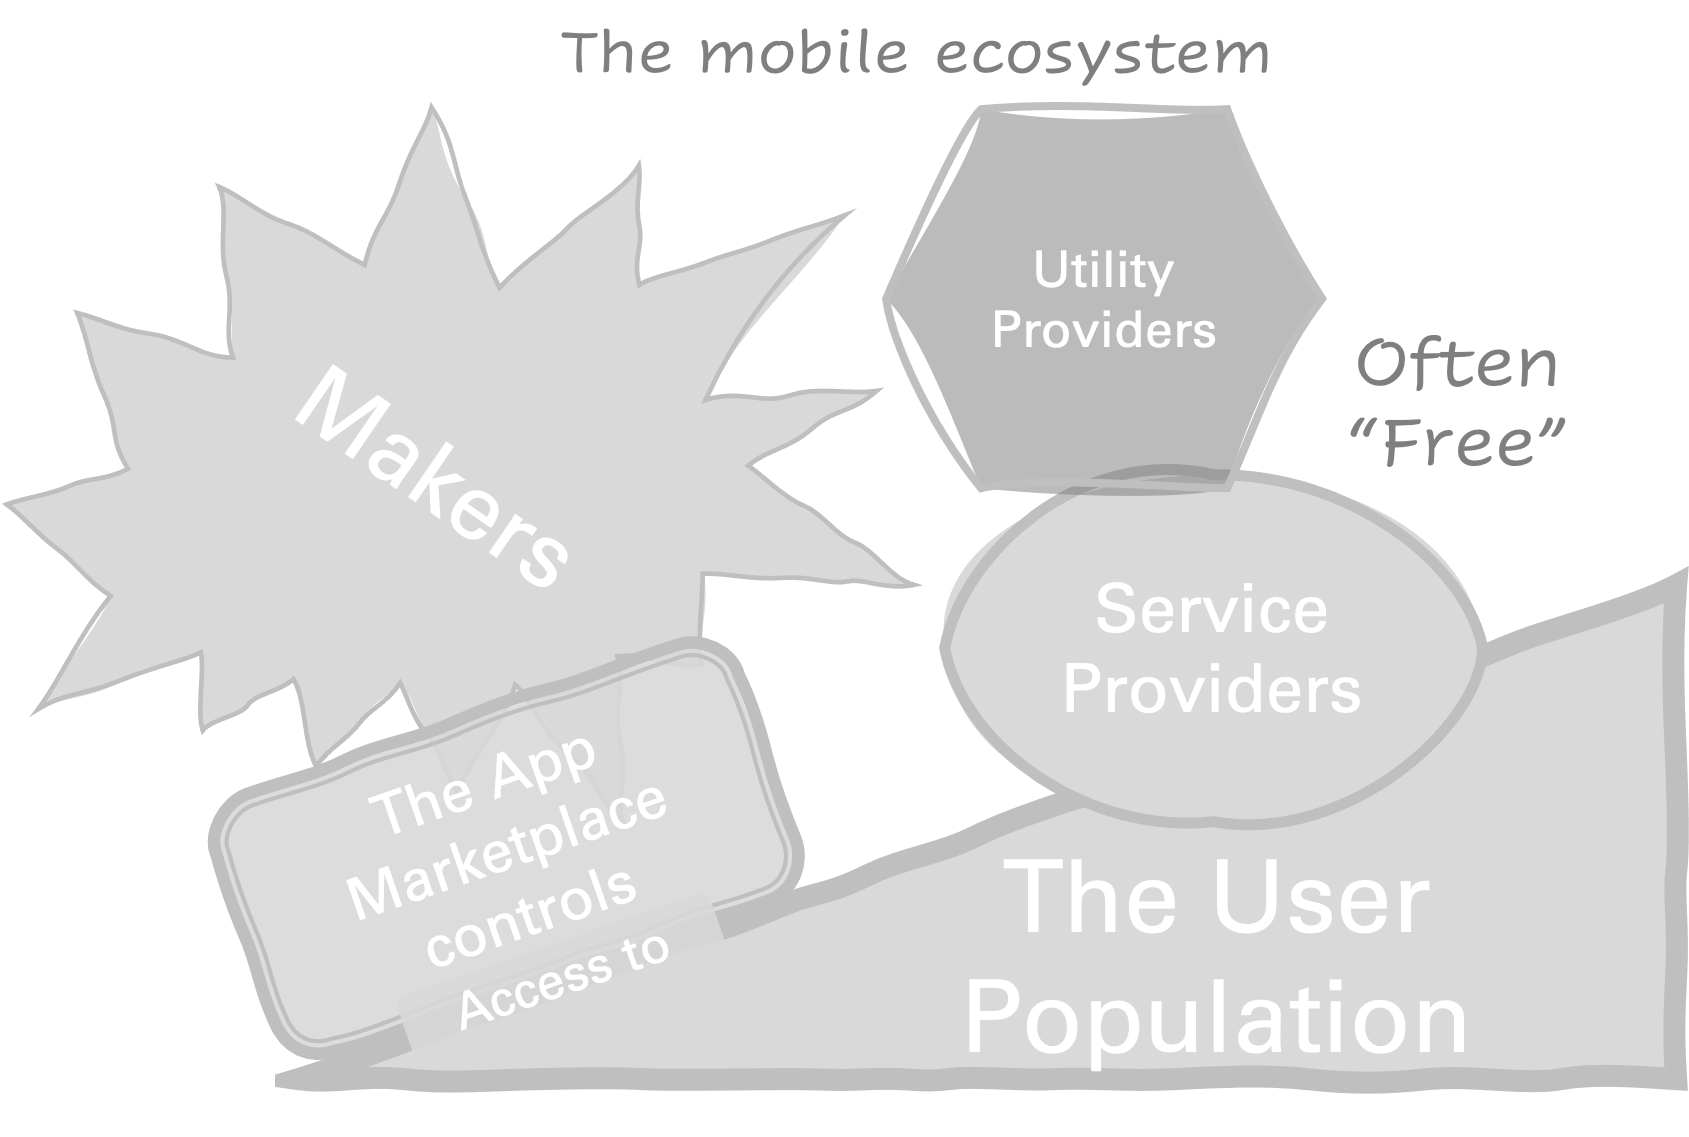
\includegraphics[width=0.8\textwidth]{images/my/the_mobile_ecosystem_sketch.png}
    \caption{The Modern Mobile App Ecosystem}
    \label{fig:my_modern-mobile-app-ecosystem}
\end{figure}

The modern mobile ecosystem, illustrated in Figure~\ref{fig:my_modern-mobile-app-ecosystem} sets the context for the thesis and this chapter together with the research questions. 
My work nestles within the works of many people in various related fields: in software quality, in analytics, and in the mobile device ecosystem. As researchers we understand and recognise there are gaps in the current state of the art, this chapter aims to identify several pertinent gaps which led to this research being performed, \emph{i.e.} which motivated me to act. The mobile ecosystems touch on billions of people's lives, where flaws in the apps and the ecosystem can adversely affect the lives of many of those people. 

Research in how mobile apps are created and tested, the relevance of app stores, service and utility providers, the user bases for mobile apps within the overall population of users of an app store ecosystem are all relevant. And meanwhile understanding why it's hard to create reliable software is also vital as part of acknowledging some of the grim realities development teams need to face if they are to succeed in their other goals and objectives for their mobile apps. An understanding of research into how to measure software qualities, and stability in particular, is key to establishing ways mobile analytics measures these qualities. At times this chapter will draw from broader sources, for instance in software development, testing, and analytics as these provide context for the particulars of the mobile app ecosystem. Conversely, in my view, and based on discussions at a peer workshop in Japan~\citep{nii_shonan_workshop_152}, I proposed a model, shown in Figure~\ref{fig:my_shonan_hysteresis_sketch}, that seemed to be well accepted and became part of the formal post-workshop report~\citep{nii_shonan_152_workshop_report}, where the mobile ecosystem is influencing the desktop app ecosystems. Examples include: app stores, per user licensing across multiple devices, public ratings and reviews, platform (device) level, crash reporting, and usage analytics, and so on.

\begin{figure}
    \centering
    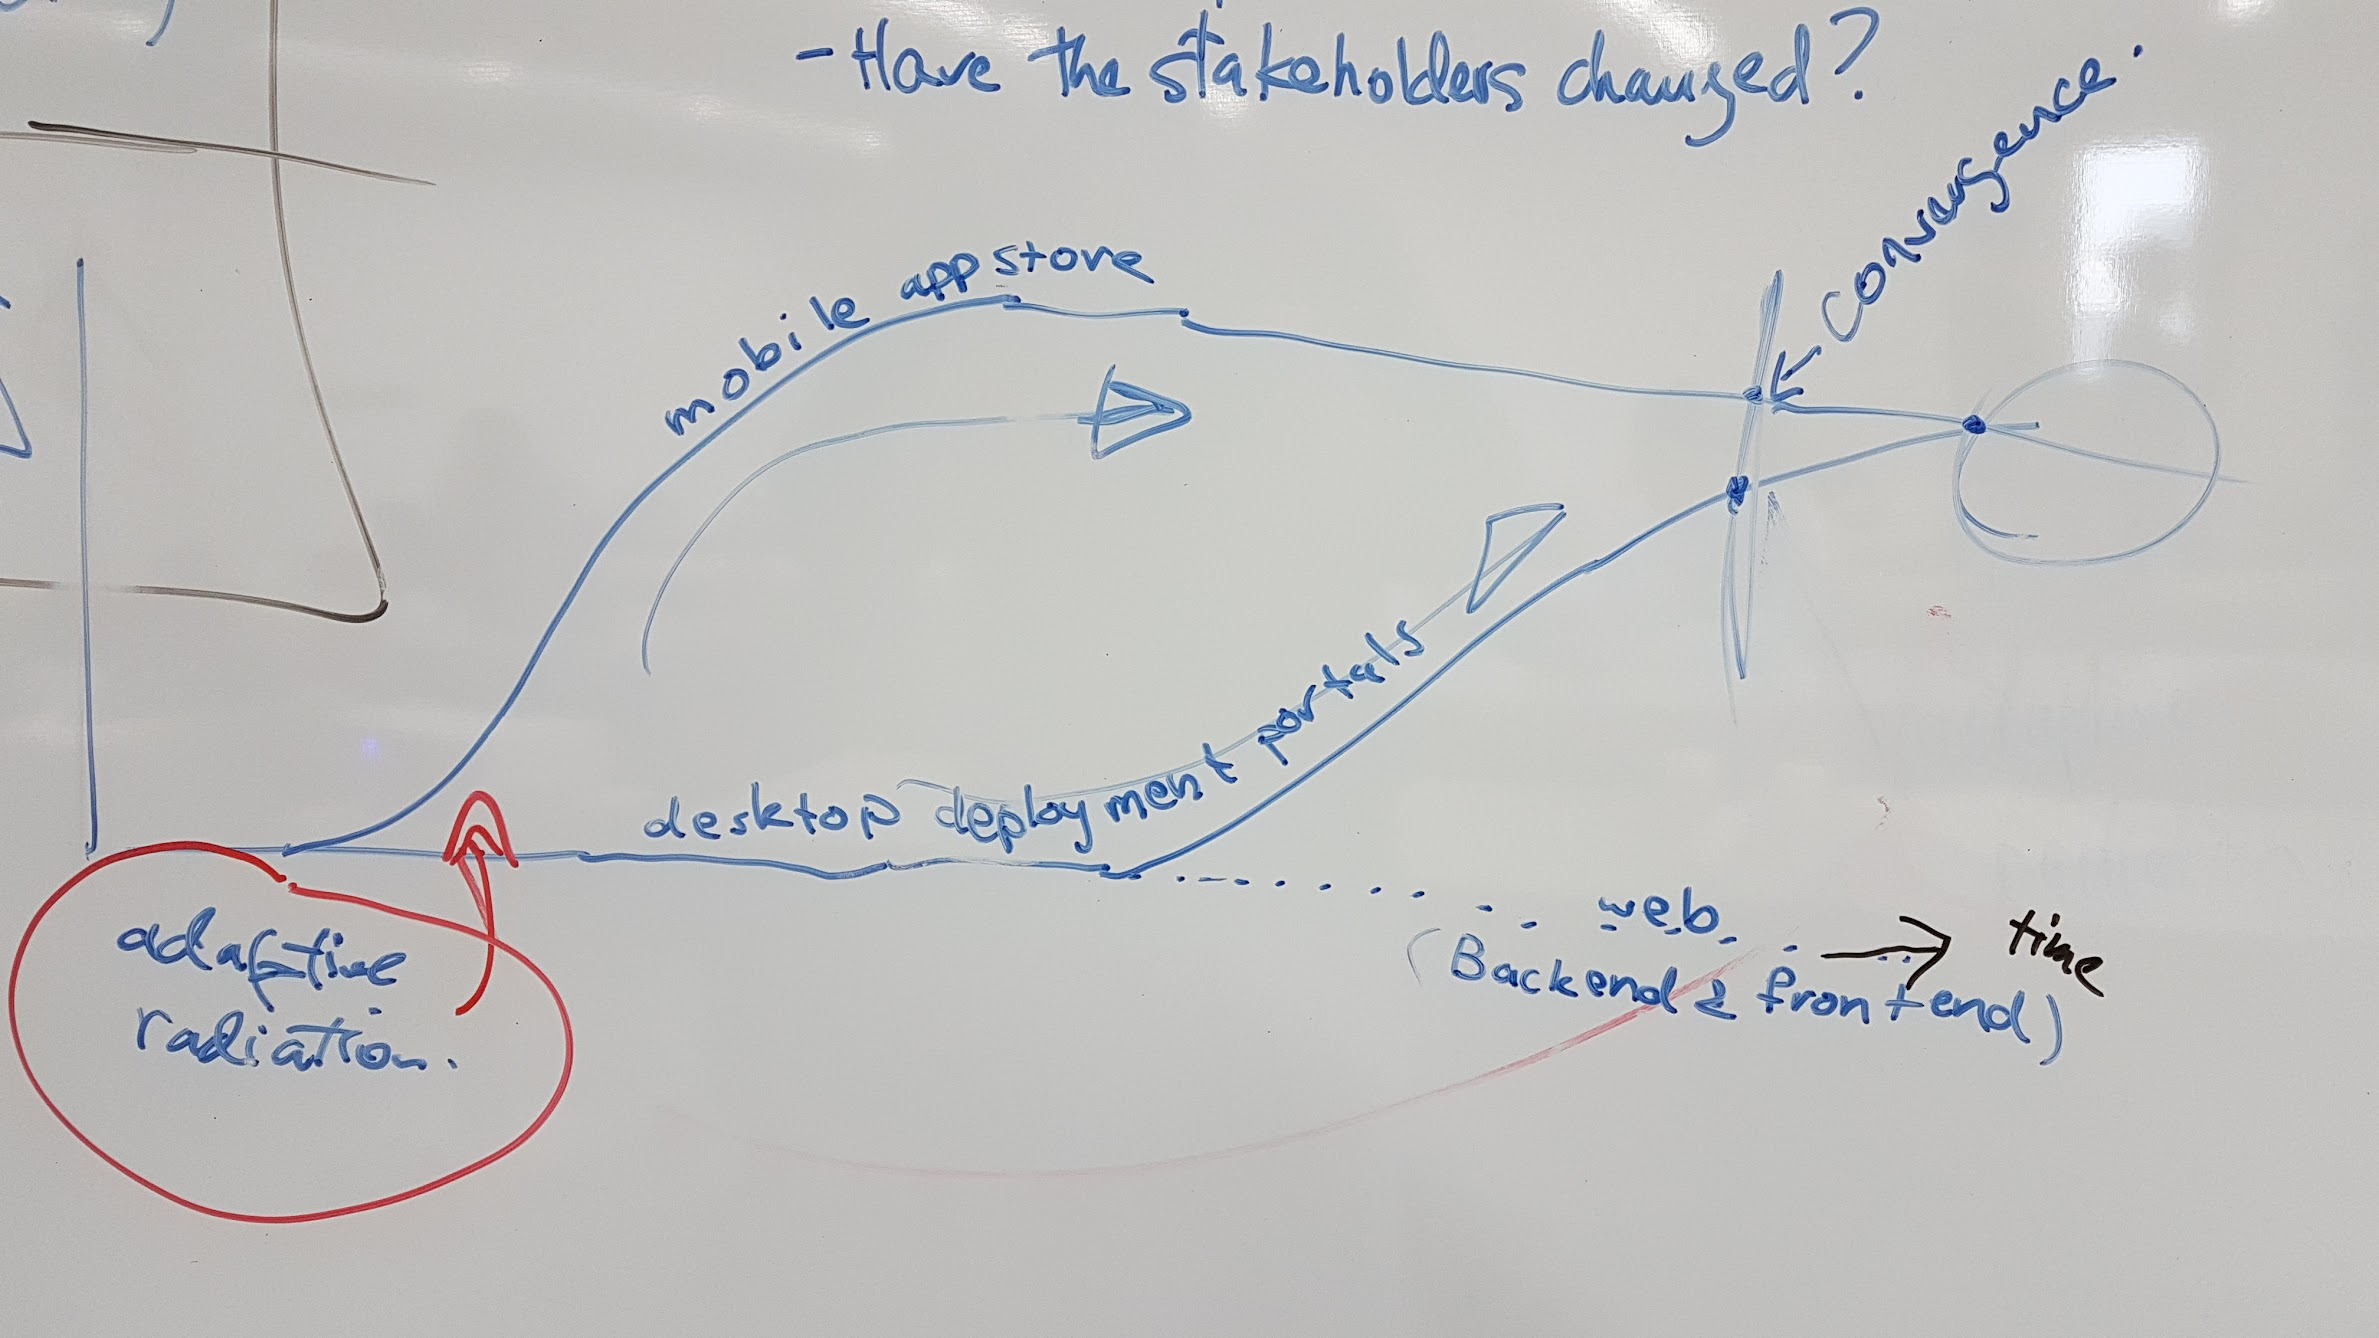
\includegraphics[width=0.8\textwidth]{images/nii-shonan-workshop-152/shonan_hysteresis_diagram_20191210_132528.jpg}
    \caption{Mobile and Desktop Growth and Convergence}
    \label{fig:my_shonan_hysteresis_sketch}
\end{figure}
.


The practicalities of the research and the case studies where nearly all the work pertains to the Google Android ecosystem also helps in the selection criteria of relevant related works. As the vast majority of active research in the domain of mobile apps also pertains to this ecosystem means the topic is richly served in terms of related works.

\section{The mobile app ecosystem}

Dated works when BlackBerry and Windows Phone app stores existed. Mainly to set the context and identify there has been plenty of research into generations of the ecosystem.


\section{Making mobile apps}
Mobile apps need to be made and developers make them. There are various working practices, apps are made by visionaries, employees, amateurs, and communities. Many claim to be ``Agile" in their working practices. There are various activities involved including development, testing, release, and deployment. Figure~\ref{fig:my_mobile-app-makers} highlights these activities as part of the overall ecosystem.

\begin{figure}
    \centering
    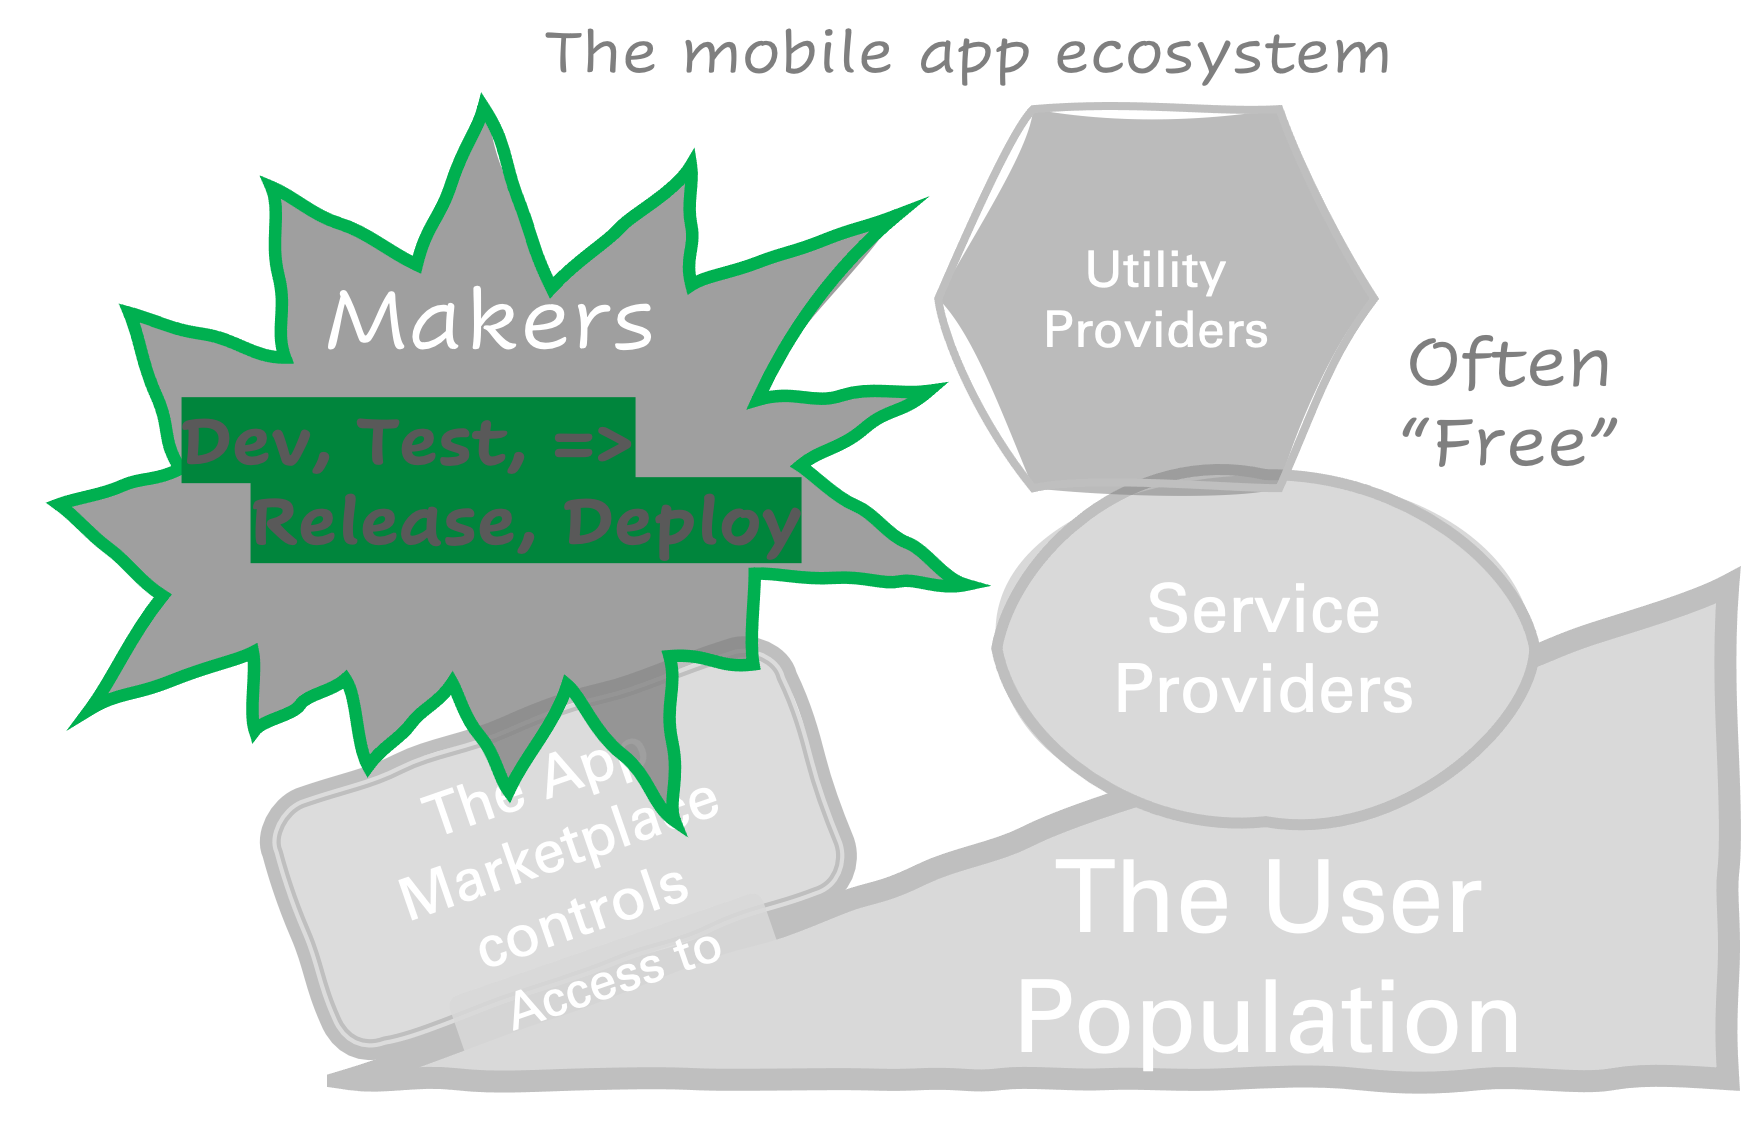
\includegraphics[width=0.4\textwidth]{images/my/the-mobile-app-ecosystem-makers-dtrd.png}
    \caption{Makers of mobile apps}
    \label{fig:my_mobile-app-makers}
\end{figure}

Unending materials are written and published online on making apps, beautiful apps, elegantly engineered apps, those that use and apply various software libraries (which we will cover in the providers section). There are a plethora of books and research materials available too. 

Books:

\subsection{Papers}

\textbf{Development practices}

Advertising in apps: 

\textbf{Testing practices}

\textbf{Code Quality: Static Analysis}

\textbf{Release and Deployment practices}

When to release an app:

\textbf{Use and efficacy of software usage analytics}: Continue the discussion introduced in the first chapter. \textit{See Isabel Evans' notes in PDF form from 4th August 2021 edition of this thesis.}

%%%%%%%%%%%%%%%%%%%%%%%%%%% End of the fresh version of this chapter %%%%%%%%%%%%%%%%%%%%%%%%%%%%%%%%%%%%%%%%
\clearpage
%%%%%%%%%%%%%%%%%%%%%%%%%%% Earlier material follows %%%%%%%%%%%%%%%%%%%%%%%%%%%%%%%%%%%%%%%%%%%%%%%%%%%%%%%

Android, given its mainly opensource codebase and popularity as a platform (Number 1 globally) is also well researched with 53 papers on the topic at ICSE 2020 and related conferences and workshops \href{https://conferences.computer.org/icse/#!/search}{ICSE 2020 Search Page}, whereas only 3 papers were on the also extremely popular iOS platform at the same set of conferences and workshops.

\begin{figure}[htbp!]
    \centering
    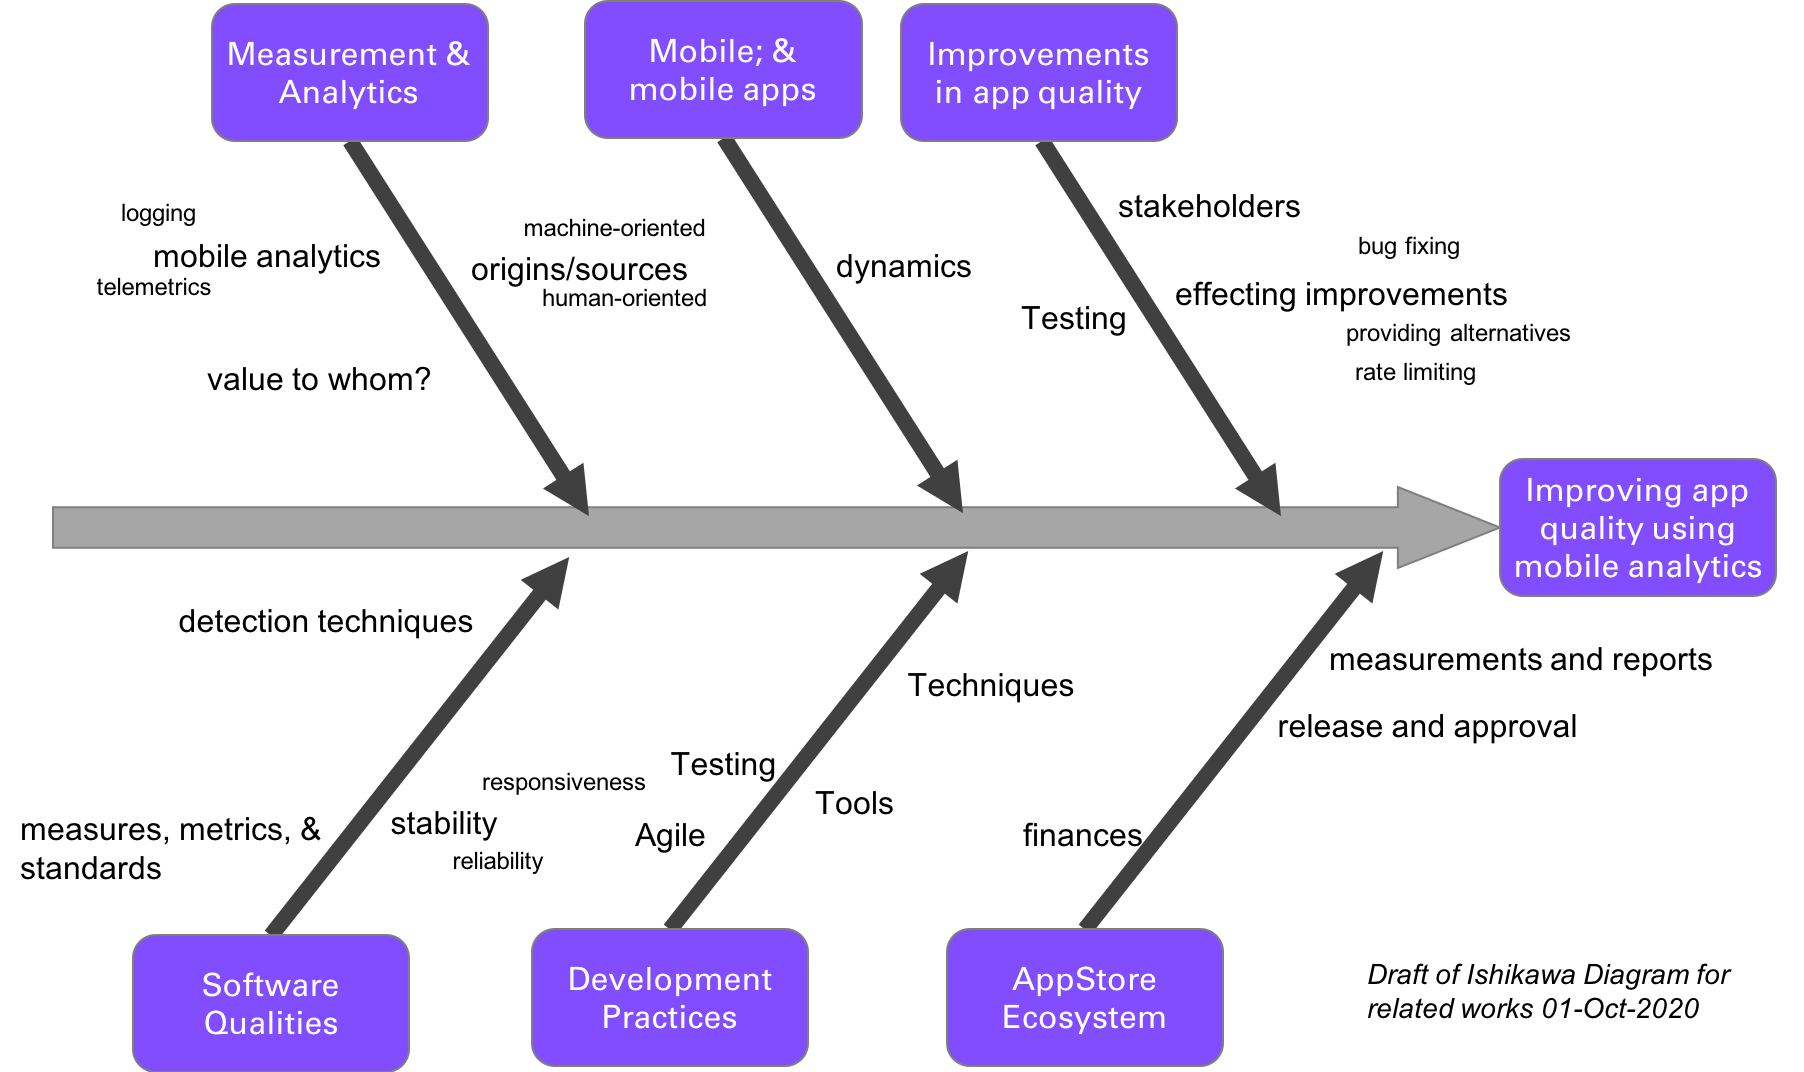
\includegraphics[width=15cm]{images/related-works-ishikawa-diagram-01-oct-2020.png}
    \caption{Ishikawa diagram for topics related to this thesis, }
    \label{fig:related_works_ishikawa_diagram}
\end{figure}

Ishikawa diagrams, also known as fishbone diagrams, can help illustrate the relationships and relevance of various topics to the overall objective. Figure~\ref{fig:related_works_ishikawa_diagram} is an example of an Ishikawa diagram for Service Support, with the aim of providing [good] quality air travel service~\cite{itil_ishikawa_example}. 
\akb{No need to provide a separate example of an Ishikawa diagram - you can explain the diagram features / notation using the diagram you've produced for your research. }
%%%%%%%%%%%%
% Learn more about Ishikawa diagrams
% https://www.moresteam.com/toolbox/fishbone-diagram.cfm 

\section{Topics to include in this chapter}
The following hierarchical list includes topics I plan to include in this chapter, after this section.


\begin{itemize}
    \item An overview on~\href{software.quality}{\emph{software quality}} including various viewpoints of quality e.g. Gerry Weinberg):
    \begin{itemize} 
        \item ISO standards
        \item Software defects, faults and failures~\hyperlink{defects.faults.failures}{\emph{link}}
        \item Bug investigation and localisation
        \item QoE: Quality of Experience
        \item Classic references e.g. Phadke~\citep{phadke1995_quality_engineering_using_robust_design} and perhaps Non-functional requirements in Software Engineering? 
        \item relevant / related academic research in my field
        \item Reliability. Introduced in ~\hyperlink{software.quality}{Software Quality}, and then expanded in a subsection~\hyperlink{software.reliability}{\emph{here}}
        \item Then focus on stability (as used by HP and then Google) encompassing reliability, freezes, etc.
        \item Discuss MTBF, usage paths and profiles and their effects on the measured values
        \item Maslow's hierarchy of needs where reliability is one of the base levels, yet vital. c.f Sommerville.
    \end{itemize}
    \item Measurement and Analytics
    \begin{itemize}
        \item Views from outside software engineering e.g. how to measure anything book
        \item Logging
        \item Telemetry
        \item Software Analytics e.g. Buse and Zimmermann
        \item Software Analytics tools and concepts e.g. free the data.
        \item Sources and mechanisms for collecting data and information about mobile apps
        \begin{itemize}
            \item Human-centric sources e.g. ratings and reviews. Perhaps also discuss some of the flaws and limitations either here or in the 'caveats...' section later?
            \item Perhaps also consider in-app feedback c.f. the Mobile Twin Peaks paper?
            \item Alpha, Beta, Crowd, and other forms of testing with subsets of a population.
            \item Program-centric sources e.g. logging, crash reporting libraries, analytics libraries, platform-level observations.
        \end{itemize}
        \item Using Data
        \item Privacy and Control
    \end{itemize}
    \item Software Development Practices
    \begin{itemize}
        \item Agile development and the effects on the software that is developed and released.
        \item Motivations for/of software developers.
    \end{itemize}
    \item Software Testing
    \begin{itemize}
        \item Schools of Software Testing? Old work that might help set the scene
        \item Classic references on software testing e.g. Boris Beizer
        \item using testing to measure quality and measuring software testing e.g. effectiveness.
    \end{itemize}
    \item App Stores and their effects on software development and engineering
    \begin{itemize}
        \item App Stores as ecosystems
        \item Release Planning (c.f DevOps and Release Engineering (including Shonan)
        \item Ratings and Reviews
        \item Google Play (and other Android app stores)
    \end{itemize}
    \item Developing mobile apps
    \begin{itemize}
        \item Single and multi-platform approaches
        \item A brief history of mobile app development
        \item Various species of bugs that affect mobile apps
    \end{itemize}
    \item Testing of Mobile Apps (this might be a distinct section in the Related Works as it's a rich topic). Do we care about testing of mobile apps that predates app store ecosystems?
    \begin{itemize}
        \item Automated testing frameworks and tools
        \item Testing practices (from both research and practical perspectives)
        \item Test Oracles
        \item Device Selection (as one aspect of testing for bug identification and investigation)
        \item Testing by crowds
        \item Measuring the efficacy of testing
    \end{itemize}
    \item Mobile Analytics~\hyperlink{mobile.analytics}{\emph{link}}
    \begin{itemize}
        \item types and sources of mobile analytics (also refer to appendix)
        \item Using Mobile Analytics to assess app behaviours
    \end{itemize}
    \item Caveats, constraints, flaws, limitations
    \begin{itemize}
        \item For instance on blind-spots, excessive trust and the ironies of automation. 
        \item Using crashes, ANRs, etc. as the test oracle - what will we miss if we only consider these aspects? how relevant is what we miss and what can we do to fill in some of the gaps?
    \end{itemize}
    \item Has anyone else published in my areas of research?
\end{itemize}

\hypertarget{software.quality}{}
\section{Software Quality}
Software quality is multi-faceted, and as the article by~\citep{kitchenham1996_software_quality_elusive_target} states, an \emph{elusive target}. This article builds on five different perspectives of quality Some facets are more user-centric, such as perceived quality by end-users, which may include aesthetics, responsiveness, brand perception, other facets focus on more technical aspects such as whether an app freezes, crashes, or whether an app corrupts, leaks, or loses data, for instance. 


I cannot hope to %or it would be impractical and potentially counter-productive to
cover all the facets even after many years of working and researching in this domain. Instead I have selected the facets germane to my PhD research.

%Expand on software quality generally before leaping into specifics.
In the 1980's and 1990's software quality became an important and established topic, with several seminal publications including:~\citep{garvin1984_what_does_product_quality_really_mean},~\citep{weinberg1992quality}, and~\citep{kitchenham1996_software_quality_elusive_target}. If we start with Weinberg who stated \emph{"Quality is value to some person"}~\cite{weinberg1992quality}. To paraphrase him, \emph{Quality is in the eye of the beholder}. For mobile apps the majority of the beholders are the end users, however the app store could also be considered a beholder, and certainly they have the power to be prosecution, judge and jury when determining which apps are allowed to be live in the app store, and which ones to promote, and which end up lower in the search results.

Considering the other two papers mentioned earlier, Garvin introduced five approaches to defining quality: 1) transcendent, product-based, user-based, manufacturing-based, and value-based. His work was extended by Kitchenham and Shari Lawrence Pfleeger. One of their key wry observations was that standards, such as ISO 9001 and ISO 9126, and maturity models, such as the Capability Maturity Model, focus on a consistent process rather than a quality product, and that~\emph{``there is little evidence that conformance to process standards guarantees good products."}~\citep{kitchenham1996_software_quality_elusive_target}. To the best of my knowledge, neither ISO standards nor maturity models figure highly for the vast majority of mobile app development teams, therefore I have considered and then chosen not to use the formal software quality models or standards in my research. 

In their discussion of the value-based view there are several foundations that were highly relevant at the time, where users were involved in product specifications and~\emph{``equating quality to what the customer is will to pay [for]"}. For mobile apps, the users are seldom involved in the specification and they do not pay with money for the vast majority of the apps they use, instead they may pay with their data... So a possible refinement of value-based views for mobile apps is to consider quality to what customers are willing to~\emph{use}? i.e. if they continue to use the app then the quality could be deemed to be adequate.

In terms of measuring quality, the authors observed,~\emph{``When users think of software quality, they often think of reliability"}~\citep{kitchenham1996_software_quality_elusive_target}. They later extend this claim and say~\emph{``[users] are also concerned about usability, including ease of installation, learning, and use."}
%
For mobile apps, these five approaches are relevant to varying degrees: development teams often internalise Agile concepts into their thinking and their practices, %MUST-DO continue this thought process here.

I will cover the both the product and manufacturing views of quality later in this thesis, particularly in several of the case studies.

% NB there is a lot more relevant and interesting material in the Kitchenham paper - see the handwritten notes on the printed copy for examples.

% \akb{You will need to choose an existing taxonomy of software quality and explain which aspects are relevant to your research before discussing literature from each of these aspects. The Kitchener et al paper below is a good starting point for this.}

In "Software Quality: The elusive target"~\cite{kitchenham1996_software_quality_elusive_target}. their work also presents two further points: The context is important when we aim to assess ``adequate" quality in a software product. And \emph{"A good definition [of software quality] must let us measure quality in a meaningful way. Measurements let us know if our techniques really improve the software, as well as how process quality affects product quality."}

%SHOULD-DO cover Quality of Experience (QoE) here. How users perceive QoE, how users communicate their QoE in an app store ecosystem, etc.

% Placed here with other material on reliability. MUST-DO Decide whether it's still needed and either integrate or remove.
Reliability is a key facet of software quality and a measure of how reliable (error-free) software is in use. Poor reliability risks jeopardising mobile apps as few users want to use an unreliable app. 
%\yijun{Why do you focus on reliability as the only facet of quality after dismissing the other facets? Do you need to worry about correctness as another quality facet related to testing?} 

As mentioned in the introduction, reliability is considered a key attribute of software quality~\citep{febrero2017_software_reliability_as_user_perception}. In their research they focus on trying to improve the understanding of an software reliability in industry. 

Maslow's hierarchy of needs~\citep{wikipedia_maslows_hierarchy_of_needs} provides a five-layered conceptual model of human needs, where lower levels dominate higher levels until they are at least partially satisfied. Reliability of software may similarly be one of the lower levels of a hierarchy of software quality, where inadequate reliability dominates until it is adequately satisfied. In some ways adequate reliability may be a hygiene factor for mobile apps and their developers. Once reliability is more than adequate developers can choose to focus more on higher level quality needs such as aesthetics as part of improving usability, and so on.

The performance and reliability quality aspects of software have been key topics for decades, including the work of Raj Jain in his seminal book~\emph{`The art of computer systems performance analysis'}~\cite{jain1991art}, a work that influenced me at the time as well as many others. One example of that influence was research into various software qualities that I and others collaborated in for over a decade, and taught and presented internationally. This included the concept of non-functional requirements and non-functional testing. Three related measures were identified related to requests for service of a computer system: performance if the request was successful, reliability if the request received an error, and availability if the request could not be performed. This is illustrated in Figure~\ref{fig:three-possible-ourcomes}~\footnote{Figure used with permission, and presented in a keynote at the StarEast 2005 conference author~\cite{harty_stareast2005_keynote}}. 

Poor reliability damages the trustworthiness and credibility of software, Ian Sommerville notes:~\emph{``... reliability was probably the most important product attribute as unreliable systems are discarded or never brought into use."}(p. 592, ~\cite{sommerville1989_software_engineering}). One of the key considerations for Sommerville is the operational reliability, and as he notes, in~\cite{mills1987_cleanroom_software_engineering}, removing software faults from seldom used code is unlikely to make a material improvement in the perceived reliability. Effective improvements need to focus on faults in frequently used code, and particularly where the failures are perceived by users of the software.

\begin{figure}[htbp!]
    \centering
    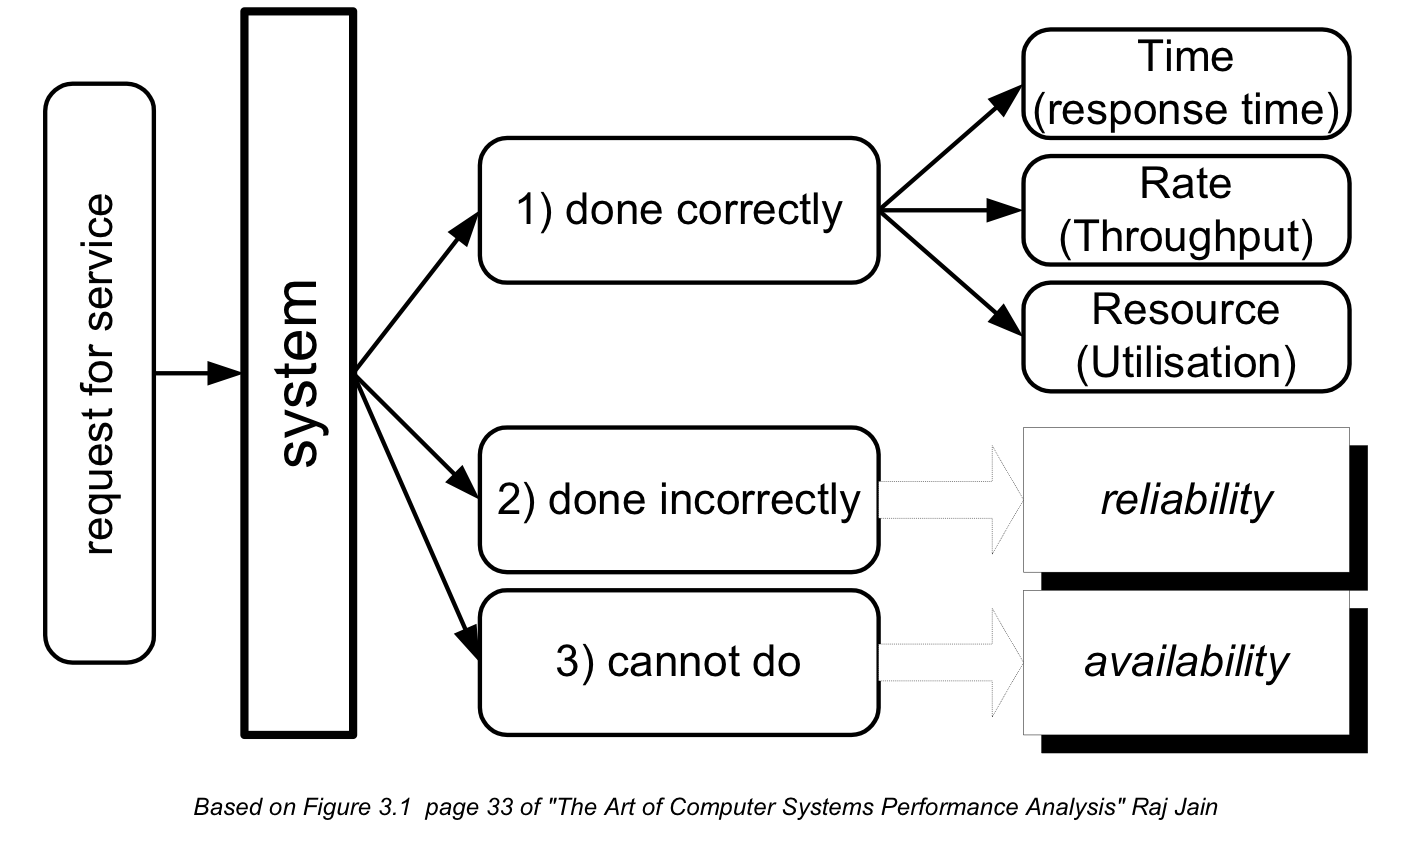
\includegraphics[width=14cm]{images/commercetest/raj-jain-performance-reliability-availability.png}
    \caption{Three possible outcomes}
    \label{fig:three-possible-ourcomes}
\end{figure}

The main software quality my research investigates is reliability as measured through counting and analysing crashes of mobile apps. While these might seem to be mundane compared to more attractive topics such as user experiences, poor reliability can undo the success of an otherwise attractive and performant software application. As Bavota~\emph{et al} observe in~\cite{bavota2014_impact_of_api_change_android} ~\emph{``users easily get frustrated by repeated failures, crashes, and other bugs; hence, they abandon some apps in favor of their competition."} Also app crashes are one of the the three most frequent complaints (together with functional errors and feature requests) found by (\cite{khalid2015_what_do_mobile_app_users_complain_about}) in their studies of 6,390 low-rated user reviews for 20 free to download iOS apps. And from a practical perspective Google states \emph{``Fixing issues can lead to a better user experience, higher ratings, and more retained installers."} in their pre-launch reports.

Crashes adversely affect reliability. They also increase the risk of users abandoning a mobile app~\citep{dimensionalresearch2015_mobile_app_use_and_abandonment}. Development teams need ways to manage risks, they also need ways to conceptualise and personalise risks according to~\citep{pfleeger2000_risky_business}. In a set of handouts paraphrases the description of risk management elegantly as \textit{``Plans to avoid these unwanted events or, if they are inevitable, minimize their negative consequences."}~\citep{amland2002_slides}~\footnote{Note: these slides are based on by a similar peer-reviewed paper of a case study that applied risk-based testing in a financial [non-mobile] application~\citep{Amland_2000_rbt_financial_case_study}.}


%\yijun{Logically I don't see the connection between quality facets => quality (general) => reliability (facet) again, perhaps you want to add some transitions so readers can follow the thoughts.}

Crash data is impersonal and oft requested and collected by operating systems and applications. For instance, when an Apple operating system is updated users are asked a couple of questions including whether they are willing to share crash data with Apple and with developers [of apps].

Unresponsive software~\emph{e.g.} when software freezes, is also problematic and may lead to poor user experiences and apps being abandoned and uninstalled. In contrast to crashes, unresponsive software may be harder to measure unequivocally. In Android Google established the term \emph{Application Not Responding (ANR)} and imbued it with distinct measurable criteria %TODO add these.



%%%%%%%%%%%%%%%%%%%%%%%%%%%%%%

The impact of various recognised forms of code refactoring has been considered in terms of internal code quality metrics for 300 opensource Android applications in~\citep{Hamdi2021empirical}. Their approach is laudable, for instance in checking the code they select belongs to live apps in Google Play. However the quality metrics they use are related to internal code quality rather than quality-in-use. As they note, the developers they studied performed many code refactorings that had no detected improvements to internal code quality. Unless the changes lead to practical improvements in the maintainability or runtime behaviours of the app, they represent an opportunity cost burden, as the developers have spent their time and energies on work that doesn't provide material improvements. In summary, this research and the underlying work published on the project's opensource site~\footnote{\url{https://github.com/stilab-ets/Android-refactoring}} provide some useful foundations for analysis of live, opensource, Android apps. However their work does not assess software qualities likely to matter to end users of these apps such as reliability, performance, UX, and so on.


\textbf{Bugs} Developers can only actively fix bugs they know about~\footnote{They may fix others inadvertently!}. Automatic collection of errors is a first step in enabling developers to learn about errors that happen at scale on end user devices. Microsoft included automated error collection in Windows XP and the challenges and practices are described in~\citep{murphy2004_automating_software_failure_reporting}. The article provides sensible and practical design considerations in terms of designing an automatic crash reporting system. Of course the world has moved on since Windows XP; and some of the advice, for instance on supporting 2-stage data collection for corporations is less applicable for mobile devices and mobile apps. 

Some bugs are hard to find and hide if they're actively sought. One type of these bugs are Heisenbugs, described in the context of Tandem non-stop computers by~\citep{gray1986_why_do_computers_stop_and_what_can_be_done_about_it}.

\textbf{Bug investigation and localisation}: A failure, such as a crash, provides a data point. A challenge of interest to both research and industrial practice is to learn enough about the failure to be able to make an actionable decision. Bug investigation and fault localisation 
are critical activities where participants frequently have various constraints they need to work within including the time they have available, the return on investment of each stage of their work, and so on.

\begin{figure}
    \centering
    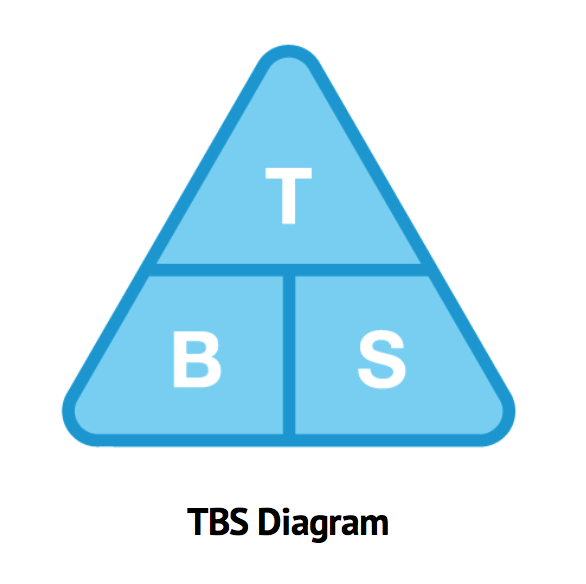
\includegraphics[width = 0.5\textwidth]{images/mobile-analytics-playbook/TBS.png}
    \caption{TBS diagram, originally in~\citep{harty_aymer_playbook_2016}}
    \label{fig:my_tbs_diagram}
\end{figure}

% c.f. T.B.S. Jon Bach
Bug investigation takes time and incurs various costs, with rare exceptions it is not done voluntarily. Repurposing and generalising Jon Bach's work on a concept he devised called ``TBS" metrics and reproduced below:

“TBS” metrics. Test design and execution means scanning the product and looking for problems. Bug investigation and reporting is what happens once the tester stumbles into behavior that looks like it might be a problem. Session setup is anything else testers do that makes the first two tasks possible, including tasks such as configuring equipment, locating materials, reading manuals, or writing a session report."~\citep{bach2000_sbtm}

A practical and systemic approach to bug investigation is available in both a book~\citep{zeller2009_why_programs_fail} and a free online course~\citep{zeller2012_udacity_software_debugging_course}. While the materials are practical, they do not include using software analytics.

\emph{``Where is the bug and how is it fixed? an experiment with practitioners"}~\citep{bohme2017_where_is_the_bug_and_how_is_it_fixed} MUST-DO continue. Similarly, `You Cannot Fix What You Cannot Find! An Investigation of Fault Localization Bias in Benchmarking Automated Program Repair Systems' has a wonderful starting title, however the bug finding techniques seem to assume the bugs are within the code of the system rather than considering external and/or combinatorial factors e.g. from the OS release, third-party libraries, firmware, timing issues, and so on. Also I'm not aware of any app developers using or relying on automated fault repair tools so perhaps that paper isn't that relevant?

Software Design and Development encapsulates the work developers of mobile apps \emph{intend} to do to create and improve mobile apps. Bug investigation and reproduction describes their focus when they are involved in understanding failure of their app. And session setup is anything else they need to do to make the first two tasks possible. Perhaps \emph{``DBS" metrics} would be a useful complement to ``TBS" metrics?

One of the arguments Jon Bach makes in various presentations is to maximise the T and minimise the B.S. This is illustrated in Figure~\ref{fig:my_tbs_diagram}.

% If practical include examples of Jon's squiggle diagrams, e.g. see slide 15 in  https://www.slideshare.net/TechWellPresentations/exploratory-testing-is-now-in-session

As many practitioners know, time spent investigating and addressing failures and related flaws in the code is time that is not available to work on features or other new stuff. As I discovered in one case study in particular, the development team may choose to only fix failures they perceive as easy to find and fix. One of the open challenges is to reduce the perceived and actual effort developers need to apply to address runtime failures in their mobile apps. 
%
Perhaps application of mobile analytics can improve bug investigation and bug localisation? 

\textbf{MUST-DO} The sources of bugs may be outside the immediate lines of code changed by developers. TBC~\citep{10.1145/3239235.3267436}



MUST-DO continue by writing about \citep{avizienis2004_basic_concepts_and_taxonomy}.


Diagnosis:

Repair: where the effort is materially less than the benefits that result from the repair. 


One of the measures applied here is using \emph{relative correctness}, a concept introduced in~\cite{diallo2015_correctness_and_relative_correctness}, ~\emph{``the
property of a program to be more-correct than another with respect to a given specification"}. The authors believe using relative correctness as a concept leads to simpler programs enhanced  in steps. This approach, of stepwise correctness-enhancing transformations, may be useful and productive in terms of using mobile analytics to improve the quality of software, and in particular the mobile apps used in our case studies. 

Research into faults and faulty programs~\cite{mili2014_on_faults_and_faulty_programs}~\footnote{And also their presentation on the topic:~\href{http://mathcs.chapman.edu/ramics2014/slides/MiliFriasJaouaRAMiCS2014.pdf}{On faults and faulty programs}} is also relevant as mobile app developers may choose to \emph{``make the program less incorrect"}~\cite{mili2014_on_faults_and_faulty_programs}. The authors also make several pertinent statements, slightly reworded from their presentation slides here for clarity:
\begin{itemize}
    \item Hypothesis: ``If a program passes the test, it is correct (fault removal confirmed)." However, the program may work when tested but fail outside [in real use].
    \item Hypothesis: ``If a program fails the test, it is incorrect (fault removal should be rolled back)." However, the program does not have to be correct; only more-correct than original. Other tests may now pass that would not have passed for the unmodified version of the program.
\end{itemize}

Improving reliability, provided it does not adversely affect other desirable qualities of a program may be considered a pragmatic and sensible option for developers, especially when they cannot guarantee their software will be fault free and they need to respond quickly to the needs of the market and their end-users.



\subsection{Seven Quality Control Tools}
Ishigawa's work extended beyond the eponymous Ishigawa, or fishbone, diagram %(as illustrated in Figure~\ref{fig:ishikawa_example_itil})
; he also devised seven basic tools for quality, in turn inspired by W. Ewdards Deming's lectures in Japan in the 1950's~\cite{7_basic_quality_tools_with_R}.

Of these seven tools, two are of particular interest in my research, his diagram to help set this work in context, and Pareto charts (also known as the Pareto distribution diagram), illustrated in one of the appendices~\hyperlink{pareto.diagrams.in.r}{\emph{here}}.


\hypertarget{defects.faults.failures}{}
\subsection{Software Defects, Faults and Failures}
\emph{Add a preamble to why this subject is relevant to my research - set this topic in context. Keep the examiner on the red thread of my research.}
\yijun{The heading doesn't match yet with the content: what about Faults and Failures? You may consider this standard for one definition:
\url{https://ece.uwaterloo.ca/~agurfink/ece653/assets/pdf/W01P2-FaultErrorFailure.pdf}}


According to Mäntylä and Itkonen more defects were found implicitly (62\%) than explicitly (38\%) ~\cite{mantyla2014_how_are_software_defects_found}, based on a survey of four software development companies in three different companies. The authors state \emph{"Implicit defect detection has a large contribution to defect detection in practice, and can be viewed as
an extremely low-cost way of detecting defects."}. Similarly my research may be considered as a useful source of finding defects implicitly, where the defects are mined and reported by mobile analytics tools and development teams can decide on the defects they deem sufficiently relevant \emph{and} practical to fix. I will discuss separately some of the implications of applying this approach to complement other approaches.

\emph{Add the take aways of why I've included this topic. Be clear about why using analytics is different from what's been done before. Explain the gaps in prior work}

~\hypertarget{software.reliability}{}
\subsection{Software Reliability}
Over twenty years ago, in a paper published at ICSE in 1997, the authors (Frankl, Hamlet, and Littlewood) discussed approaches to select testing methods to deliver reliability. They identified two main goals in testing software: 
\begin{enumerate}
    \item to \emph{achieve} reliability~\cite{frankl1997choosing_testing_for_reliability} (using testing to probe software for bugs so they could be removed to improve the reliability), and 
    \item to \emph{evaluate} reliability, an approach they call \emph{operational testing}, where tests reproduce the expected usage of software and testers wait for failures to occur.
\end{enumerate}

Both approaches provide a mixed bag of desirable and undesirable effects; in the paper the authors compare the testing effectiveness based on the reliability of the program after it was tested. In their conclusion they state: \emph{"research cannot offer decision makers a best testing method for all situations."}. Instead they believe research can offer better criteria for informing the choice of a method to suit a decision maker's specific situation. They also hope to guard against, and help people avoid, illogical decisions.

Their work intersects with the work of Dorothy Graham's proposed measure of Defect Detection Percentage (\emph{DDP}, for short)~\cite{graham_measuring_2009} aimed at evaluating the effectiveness of whatever testing was performed by comparing the issues found during testing with those found subsequently, often when the software is in use by others.

Frankl, Hamlet, and Littlewood discussed operational testing based on expectations of the inputs; in turn a paper by Bishop in 1993~\cite{bishop1993variation} discussed the variation in software survival time depending on differences in the operational input profiles. Failure probabilities are not constant, the paper states the probability of failures decreases as the time from the last failure increases. There are several relevant observations in the paper, including: \emph{"During a failure, restarting the software will have little effect if the input conditions are similar..."} for instance a mobile app may crash repeatedly if a user (for instance) happens to repeat an action that exercises the code that fails. This was observed this behaviour in Kiwix, one of the Android apps under evaluation, where a single crash occurred 55 times for a single user, as Figure~\ref{fig:55-crashes-missing-webview-package-exception}.
%\yijun{It is good to confirm the points in your observation.}

\begin{figure}[htbp!]
    \centering
    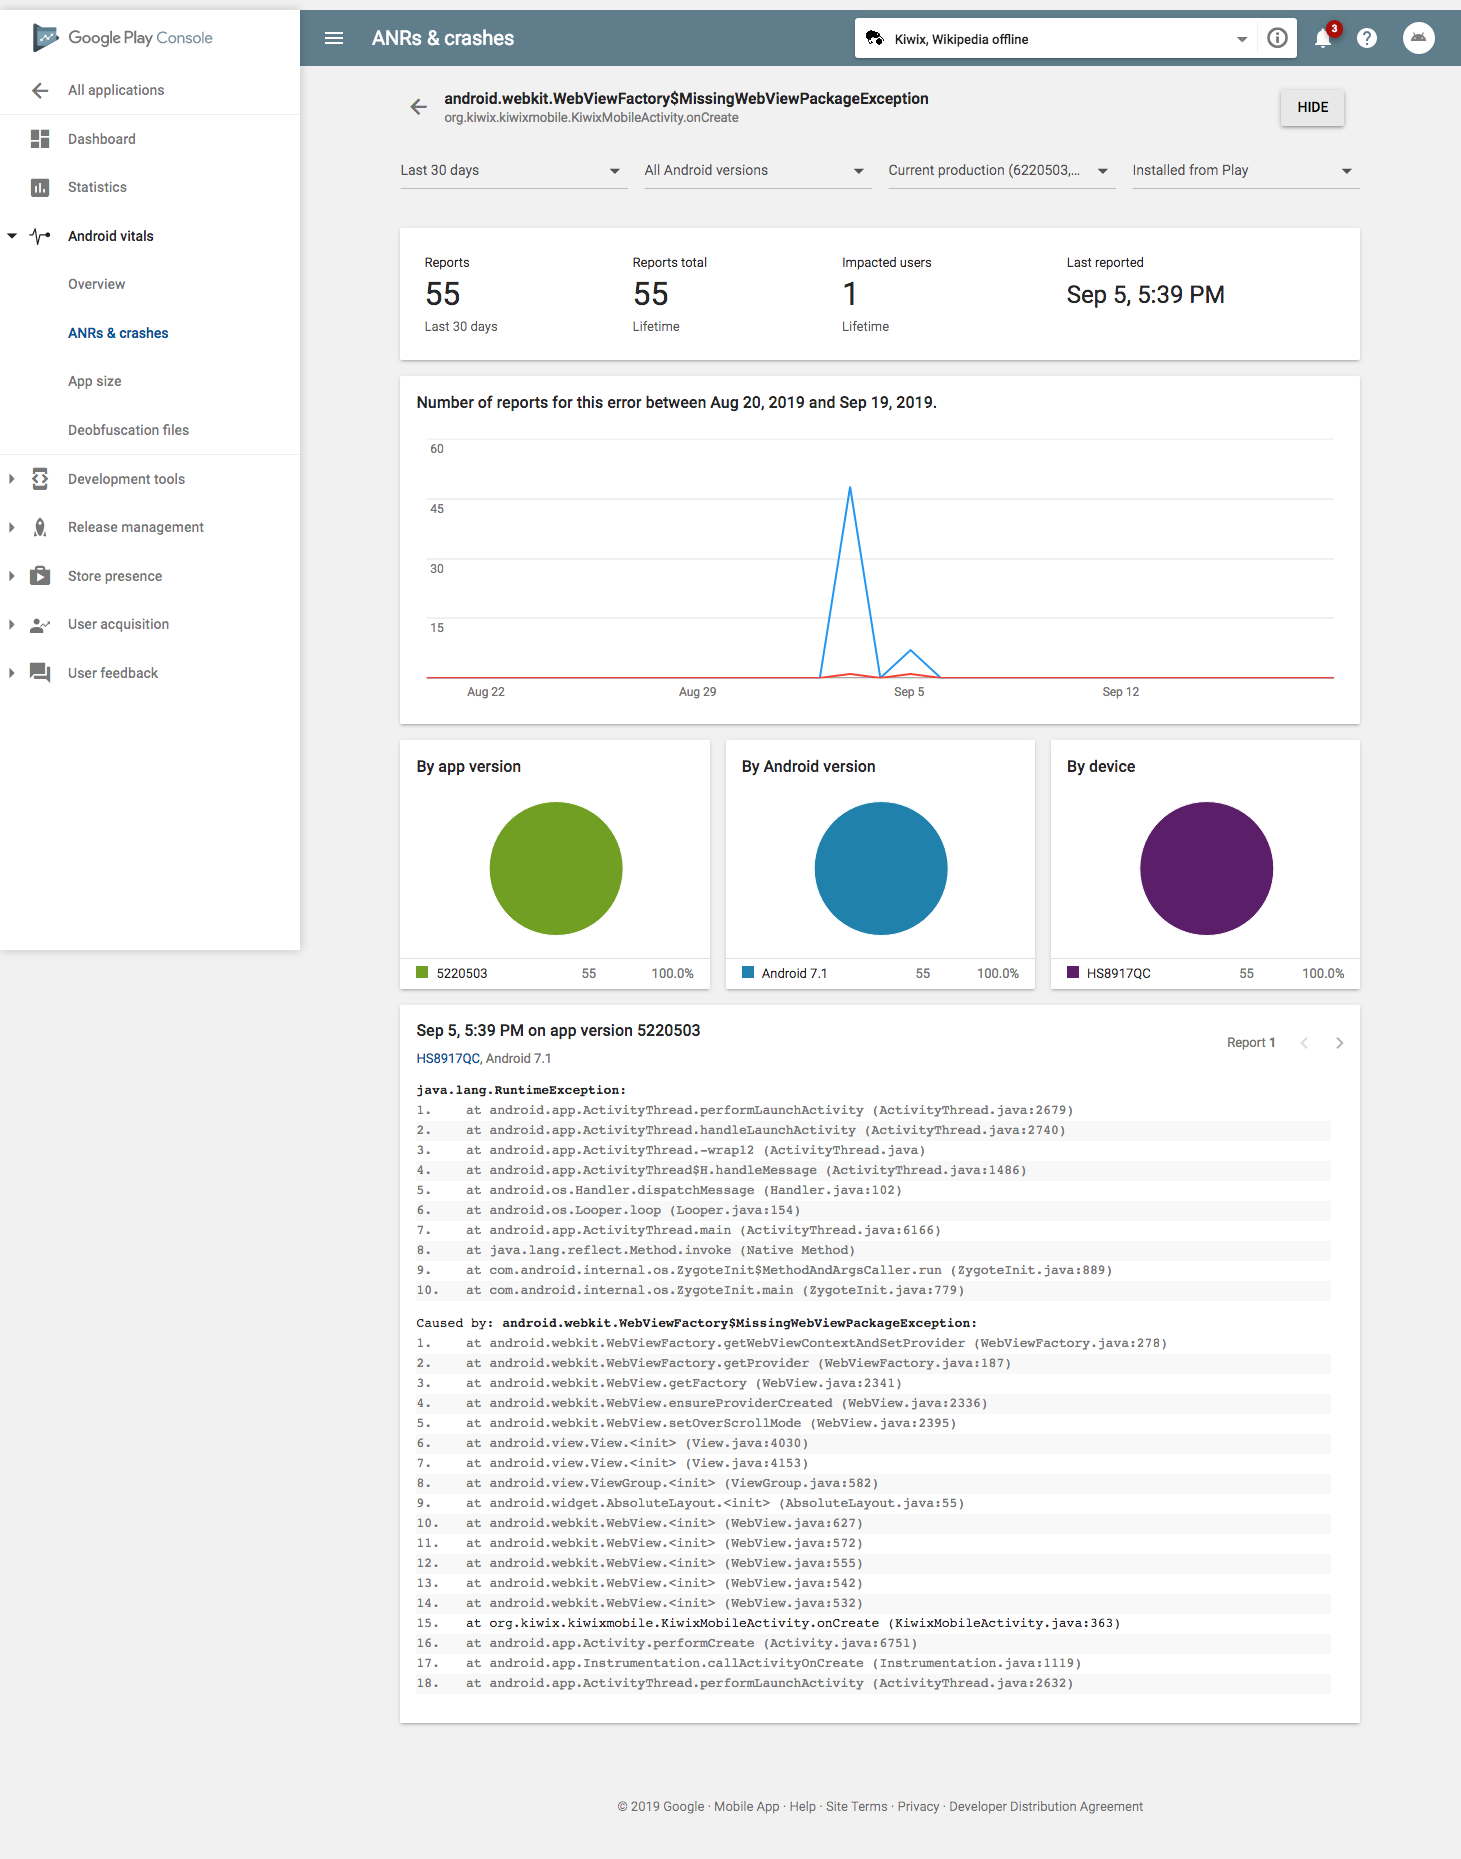
\includegraphics[width=14cm]{images/android-vitals-screenshots/55-crashes-WebViewFactory-MissingWebViewPackageException Screenshot_2019-09-19-kiwix.png}
    \caption{Google Play Console: Missing WebView Package Exception}
    \label{fig:55-crashes-missing-webview-package-exception}
\end{figure}

Another result from the paper is: \emph{"Given that the software is operating successfully, the chance of continued operation is greatly improved if there are only small changes in input conditions..."}. For mobile apps, one of the ongoing, major, sporadic changes are to the version of the operating system. As Linares \emph{et al} ~\cite{linares2013_api_change_and_fault_proneness_android} found, the most frequent cause of failure for Android apps is when the operating system is updated. Apps that were reliable on previous releases of the operating system may now start failing, and some failures become frequent and widespread as the new operating system release is adopted. \textbf{MUST-DO add evidence on the rollout and growth of Android releases in use as per old Google Android charts.}
~\yijun{This is very true in the TM352 I experienced. An argument may lead to the gap analysis is: how can one control or limit the effect of such external change factors or live with it? Is mobile analytics towards living with it while presenting an opportunity to spot such incompatibility issues earlier? }

These existing works help to establish the importance of reliability, some of the ways testing can be evaluated in terms of the subsequent reliability of the software in use, and some of the challenges in finding bugs that affect reliability. 

Another classic paper, from 1993, is by Musa~\emph{``Operational profiles in software-reliability engineering"}~\cite{musa1993_operational_profiles} which proposed using an operational profile to guide testing to maximise testing of the most-used operations. For mobile apps a key challenge, firstly there's unlikely to be a single operational profile for many apps given the variety of ways users use those apps how many would be needed to provide adequate coverage? and secondly where does the underlying information come from to determine what the operational profiles need to be in order to test effectively and efficiently? Musa does discuss ways to record the data: potentially Mobile Analytics may help to provide the data needed to establish these operational profiles? 

\textbf{TODO} sum up this section and connect it with Google's concept of Stability metrics to measure software quality for Android apps.

\subsection{Additional papers to consider on software quality}
These have not yet been incorporated into this section on Software Quality.
\begin{itemize}
    \item Sources of taxonomies and software testing include:~\cite{foidl2018_integrating_software_quality_models_into_risk_based_testing} 
    \item ``Cornering the Chimera"~\cite{dromey1996_cornering_the_chimera}.
    \item ``An Empirical Study on Quality of Android Applications written in Kotlin language"
    \item ``Mining Non-Functional Requirements from App Store Reviews"

\end{itemize}

\section{Measurement and Analytics}

\begin{figure}[!htbp]
    \centering
    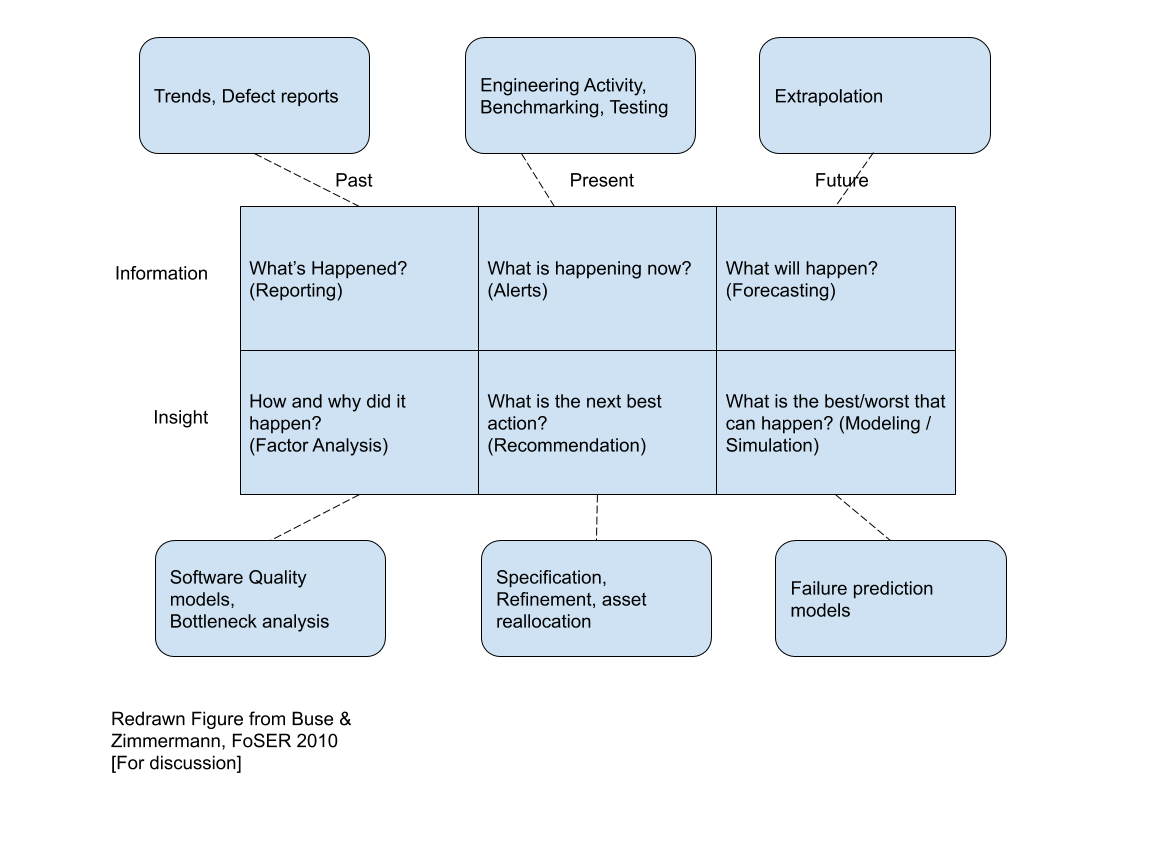
\includegraphics[width=14cm]{images/Buse_and_Zimmermann_2010_figure.png}
    \caption{Software Analytics, Buse and Zimmerman (2010)}
    \label{fig:software_analytics_buse_and_zimmerman_2010}
\end{figure}

Buse and Zimmerman wrote a short paper in 2010 which helped establish the field of:~\emph{``Analytics for Software Development"}~\citep{buse_analytics_2010}. The first figure in that paper is reproduced here as~\ref{fig:software_analytics_buse_and_zimmerman_2010}. They had derived that figure from a more general business-focused diagram in Davenport and Harris's book~\emph{``Analytics at work: Smarter decisions, better results"},  in Figure 1.1, titled\emph{``Key questions addressed by analytics"} and found in page 7 of ~\citep{davenport2010analytics_at_work}).

\begin{figure}[!htbp]
    \centering
    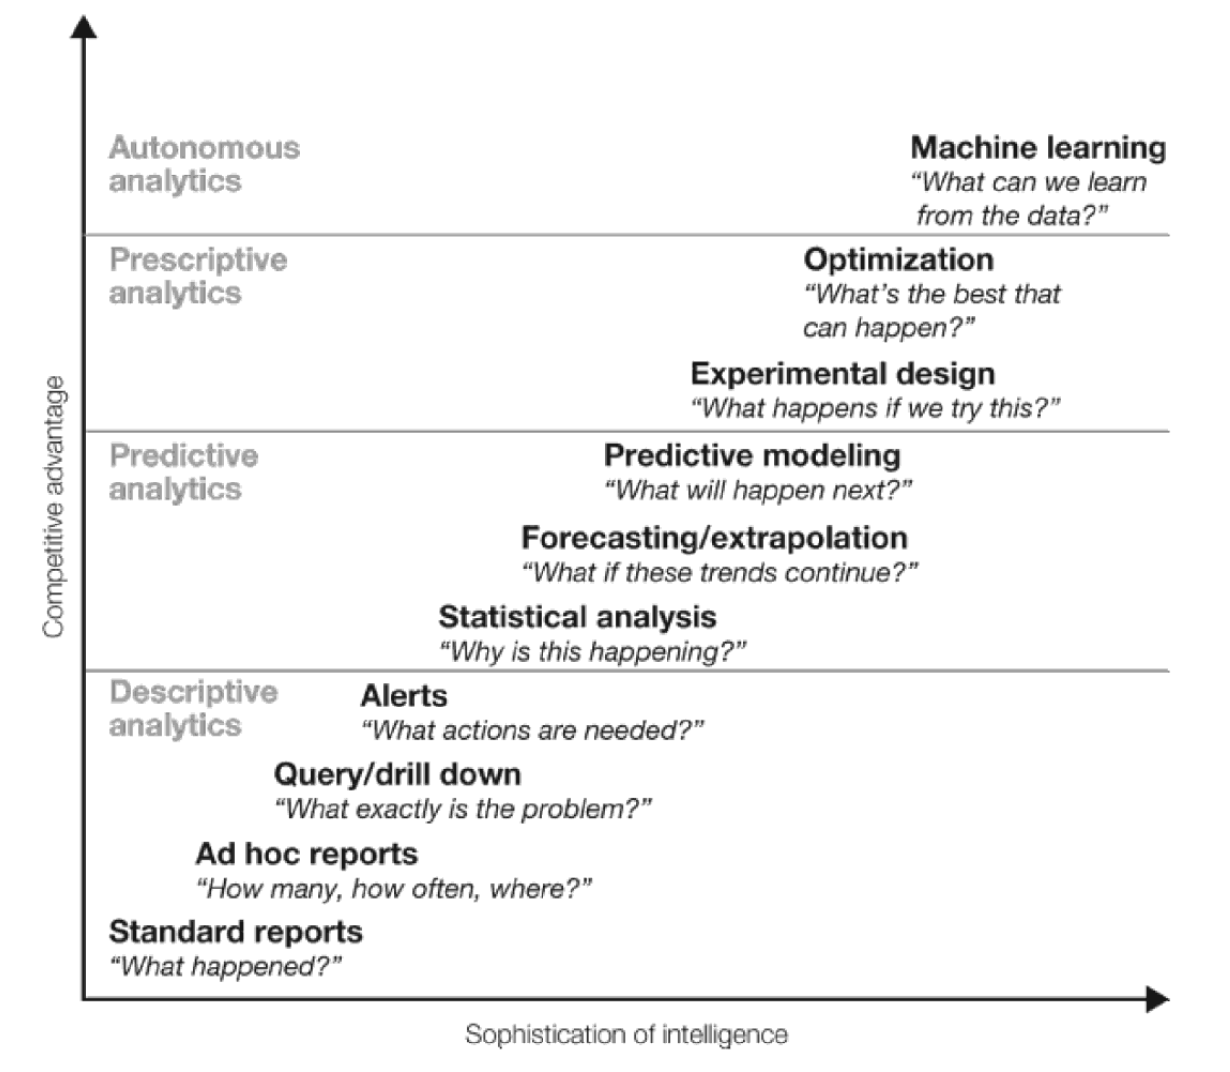
\includegraphics[width=14cm]{images/hbr/davenport-et-al-competing-on-analytics-2017-competitive-advantage.png}
    \caption{Davenport et al. Analytics for Competitive Advantage}
    \label{fig:davenport-analytics-for-competitive-advantage}
\end{figure}


\subsection{References/Sources to consider}
\begin{figure}
    \centering
    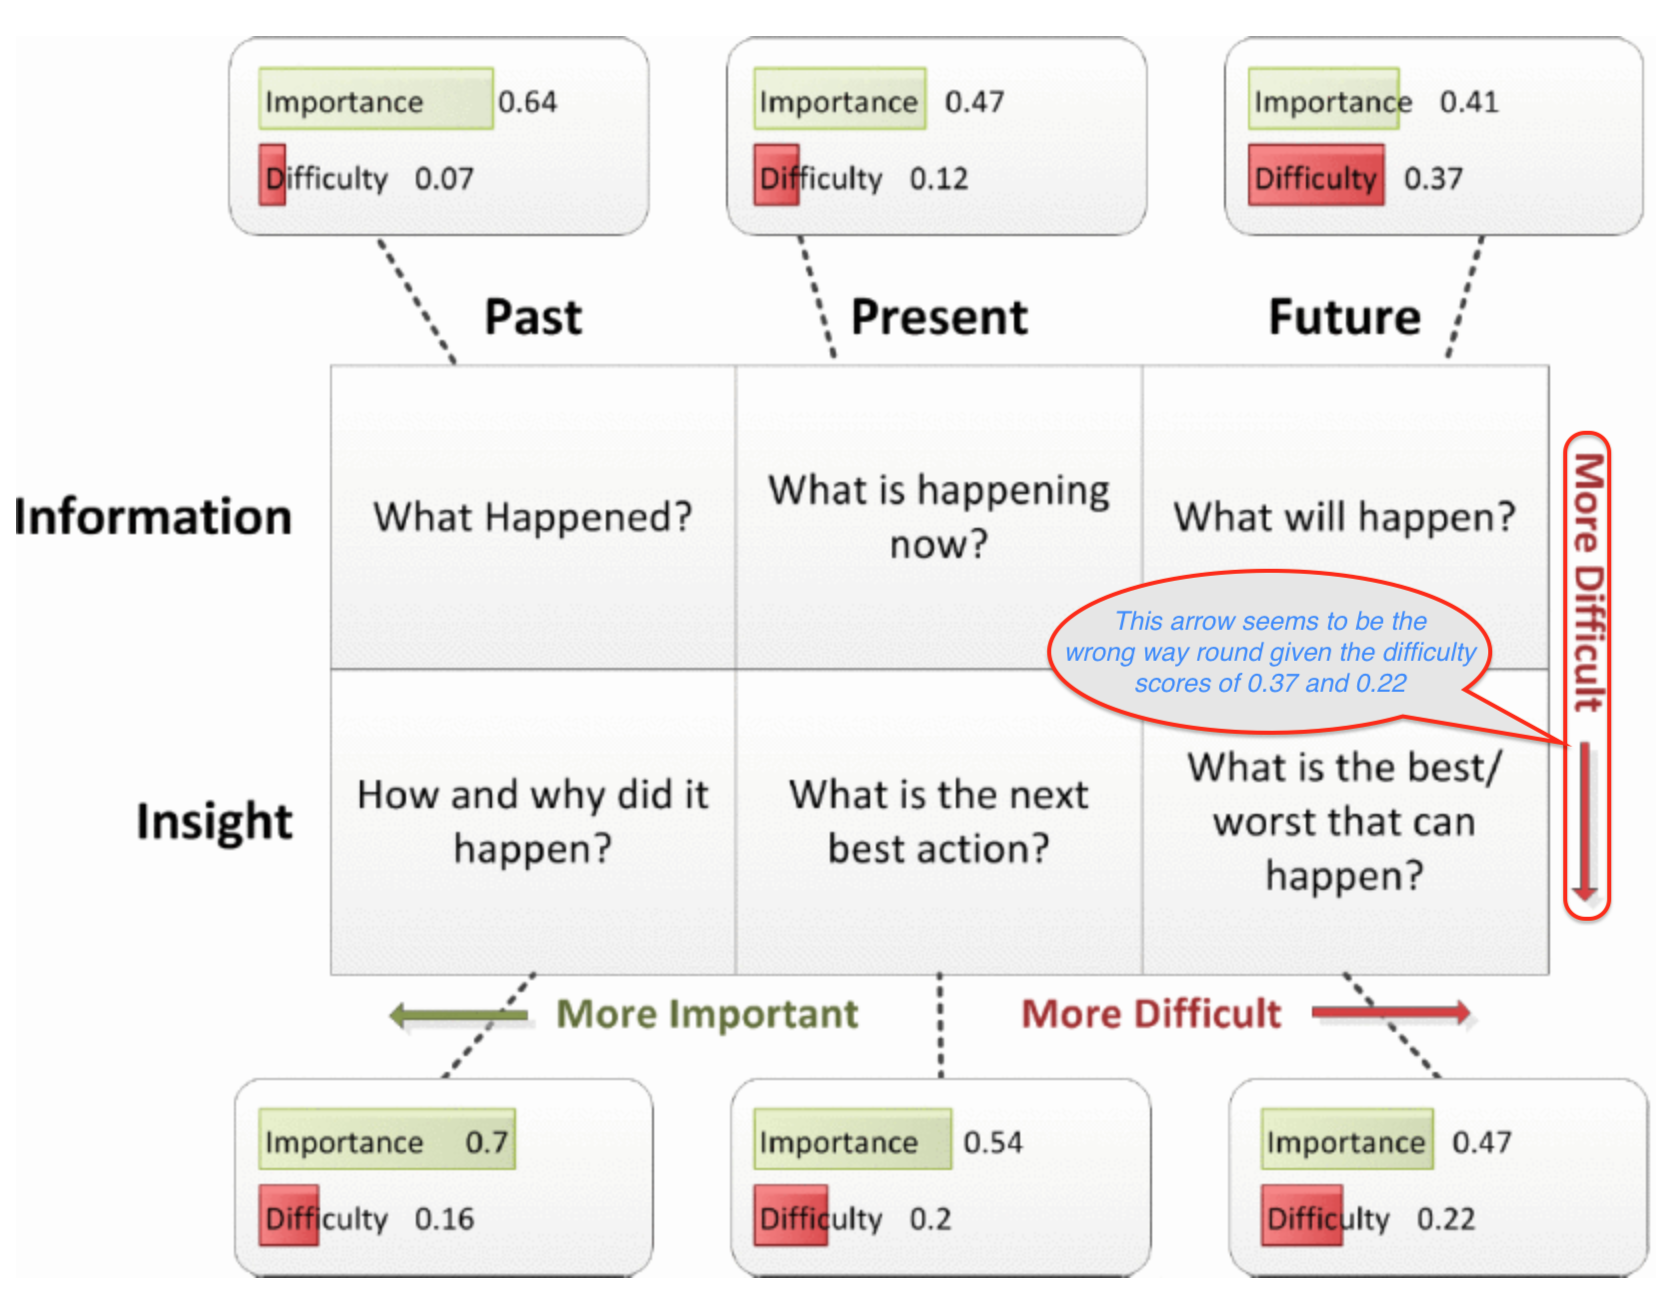
\includegraphics[width=13cm]{images/related-work/buse2012-edited-figure-2.png}
    \caption{Revised Figure 2 from~\citep{buse2012_information_needs_for_software_development_analytics}}
    \label{fig:buse2012-edited-figure-2}
\end{figure}
\begin{itemize}

    \item \emph{``Capturing Mobile Experience in the Wild: A Tale of Two Apps"}~\citep{patro2013_capturing_mobile_experience_in_the_wild}. Also mention the respective GitHub projects \url{https://github.com/patroashish/InsightClient} and \url{https://github.com/patroashish/InsightServers}.

    \item Davenport \textit{et al.} Competing on Analytics (\cite{davenport2017competing_on_analytics}) figure 1. Note: Google with version 4 of Google Analytics, launched in October 2020, are offering some machine learning based analytics to their customers, for instance to help marketeers... TBC. MUST-DO continue this topic and provide references to sources.
    
    \item Davenport \textit{et al.} Competing on Analytics (\cite{davenport2006competing_on_analytics}) that proposes several related functions: understanding customers and their contexts (including equipment and settings), product and service quality \emph{``detect quality problems early and minimise them"}, and to \emph{``improve quality, efficacy, and, where applicable, safety of products and services"}.
    
    \item \emph{``Charting the API minefield using software telemetry data"}~\citep{Kechagia2015_charting_API_minefield_using_telemetry_data}. The stability of Android apps has been measured using telemetry data collected by a centralised crash report management service. Roughly one million stack traces were analysed from thousands of Android applications. A subset (over 500,000) of these stack traces were associated with risky API calls and these were analysed to identify the most common failure reasons. The top five reasons were attributed to:
    \begin{itemize}
        \item memory exhaustion,
        \item race conditions,
        \item deadlocks,
        \item missing resources, and
        \item corrupt resources.
    \end{itemize}
    The authors provide a set of recommendations they claim \emph{may} help address various classes of the crash failures. However these recommendations do not appear to have been tested for their efficacy. Their recommendations are theoretical rather than practical. There's an odd claim in the paper in page 1818, \emph{``In addition, the platform of Chen et al. (2011), which is based on remote resource management, can make applications require less memory and resources. Hence, it can eliminate the well-known “non-responsive” exceptions in Android."}. For this claim to hold true \textbf{all} the causes of non-responsive exceptions (or did the authors mean ANRs? they don't define this term or use it elsewhere in the paper) would need to be a) related to remote resources, and b) the difference would need to be directly related to the amount of memory and resources. Google provides five common patterns for diagnosing ANRs~\footnote{\url{https://developer.android.com/topic/performance/vitals/anr\#diagnosing_anrs}} none of these mention remote resource management (even if they may contribute to ANRs). The authors say in the introduction to section 5.1~\emph{`API Recommendations'}, on page 1813,~\emph{``Finally, we provide the frequencies of the representative signatures to show how many crashes could be avoided based on the following solutions."}, however they did not appear to provide this unless they are the charts in  Appendix 1 \textbf{\textit{and}} if their proposals solve \textit{all} the causes of the crashes in each category. This was promising, thought-provoking, and interesting work which sadly lacked evidence their proposed recommendations actually work in practice for any of the apps that provided the crash data or for other Android apps (if their work is generalisable).

    
    \item \emph{Software Telemetry (MEAP)}~\citep{riedesel2020_software_telemetry_meap_v04}. An early draft of a book scheduled to be published in mid 2021 that discusses telemetry including the roots in system logs on early computer systems.
    
    \item \emph{``Software Analytics, so what?"}~\citep{menzies2013_software_analytics_so_what} to set the context.
    
    
    \item Buse and Zimmermann...~\cite{buse_analytics_2010} e.g. \emph{“We distinguish between questions of information which can be directly measured, from questions of insight which arise from a careful analytic analysis and provide managers with a basis for action.”}
    
    \item \emph{``Information needs for software development analytics"}~\citep{buse2012_information_needs_for_software_development_analytics}. They asked 110 Microsofties, a mix of development leads and managers about their use of software development analytics. MUST-DO discuss how my work and their guidelines for software development analytics align. What does my work add to their work? What does it provide that they identified back in 2012? Their focus seems to be more on the code than the product of the code (apps and the services (and the qualities of those services) those apps provide to end users). What information do mobile app developers need in terms of improving the reliability of their apps? How can the developers make good decisions in this area?
    \begin{itemize}
        \item ~\emph{``we ultimately want to} empower software development teams to independently gain and share insight \emph{from their data without relying on a separate entity"}
        \item \emph{``Analytics can help: monitor a project; know what's really working; improve efficiency; manage risk; anticipate changes; evaluate past decisions."}
        
        \item Oddly, Figure 2 in their paper seems to have a mistake in the direction of More Difficult from Information to Insight, see~\ref{buse2012-edited-figure-2}.
        
        \item \emph{``In other words, both developers and managers find it more important to understand the past than try to predict the future; echoing George Santayana, “those who cannot remember the past are condemned to repeat it.”"}.
        
        \item From Figure 4 in their work, Failure Information (\emph{``reports of crashes or other problems"})is in the top 3 that the development leads would use and top for managers when making decisions relevant to their engineering process. Telemetry (\emph{``user benchmarks"} would be used by around 80\% of development leads and 90\% of managers in the survey.
        
        \item \emph{``The landscape of artifacts and indicators in software engineering is well known, but the concrete decisions they might support are not. We conjecture that understanding how managers and developers can make use of information is critical to understanding what information should be delivered to them."}. My research somewhat inverts this by looking at what's being delivered in terms of commercial, pre-existing mobile analytics and considers how that information has been used to improve the reliability of the mobile apps that were the source of the raw information.
        
    \end{itemize}~\citep{buse2012_information_needs_for_software_development_analytics}.
    
    \item The data collection and analysis of Android Vitals has some similarities with Microsoft's `Windows Error Reporting' (WER) which they describe in an article in 2011~\citep{kinshuman2011_debugging_in_the_very_large} and a longer conference paper from 2009~\citep{kinshuman2009_debugging_in_the_very_large}. Similarities include both mechanisms being designed to work effectively at scale of at least a billion end-user machines/devices, capturing crash data, and using error statistics as a tool in debugging. Differences include the platform (Android), the lack of automatic diagnosis (which WER provided), and most relevantly, Google provides several million third-party developers with access to data for the apps they are responsible for and provides them with various comparative analytics of the technical performance of their app compared to those apps of their peers. (Microsoft provided 700 third-party developers, for instance of device drivers, with WER information, and the paper provides a concrete example of how one vendor addressed the top 20 reported issues for their code, and how the fixes percolated out to the end users and halved the percentage of all kernel crashes attributed to that vendor (from 7.6\% to 3.8\%)).
    
    \item An opensource project provides Android developers with a mechanism to detect and report ANRs in their application. It includes support to report the ANRs to various crash reporters~\citep{salomonbrys_github_anr_watchdog}. (Two of the four listed (Crashlytics and HocketApp) have been acquired by Google and Microsoft respectively). Note: In 2012, Google was asked to provide a facility to detect ANRs from the application~\footnote{\url{https://issuetracker.google.com/issues/36951741}} so developers would be aware of them and be able to address them. The issue was marked obsolete by Google in 2014 without comment. A similar reporting feature is now available in Android on Google supported devices.
    
    \item \emph{``Challenges and Benefits from Using Software Analytics in Softeam"} ICSEW 2020 \emph{``In this industry abstract, we describe the challenges and benefits of collecting feedback from customers and systems to support development cycles. In Softeam, we have performed such collection and support in four iterations by means of a software analytics platform. We describe the encountered challenges and the effects of suggested recommendations to improve the software quality of our systems on the metrics of interest."}~\cite{bagnato2020_challenges_and_benefits_from_using_software_analytics_in_softeam}. They use \url{https://github.com/q-rapids}, a ``Quality-aware rapid software development. H2020 Project (Grant no. 732253)". There are relevant publications listed at \url{https://www.q-rapids.eu/publications}.
    \item \emph{``"} \emph{``automatically collected usage data, logs, and interaction traces could improve feedback quality and help developers understand feedback and react to it. We call this automatically collected information about software usage implicit feedback."}~\citep{maalej2016_towards_data_driven_requirements_engineering}. They claim~\emph{``Thermal tracking of a user’s finger movement on touchscreens is a common approach for usage data analysis."} however I'm not aware of evidence to support this claim either from a research or a practitioner's perspective. (There's a PhD thesis on this topic published \emph{after} this paper: \href{http://usir.salford.ac.uk/id/eprint/37784/}{`Investigating the usability of touch-based user interfaces'}.
    
    \item ``A Methodology and Framework to Simplify Usability Analysis of Mobile Applications" Adding logging to a mobile apps can help developers analyse usability, reducing the effort needed
    
    \item \emph{``How Does Misconfiguration of Analytic Services Compromise Mobile Privacy?"} ICSE 2020. This in turn refers to \emph{``Alde: privacy risk analysis of analytics libraries in the android ecosystem."} 2016, and \emph{``Bug Fixes, Improvements, ... and Privacy Leaks - A Longitudinal Study of PII Leaks Across Android App Versions."} 2018.
    
    \item \emph{``Prochlo: Strong privacy for analytics in the crowd"}  ~\citep{prochlo2017_strong_privacy_analytics_in_the_crowd_46411} Various Google authors. 2017. Quote from the abstract:~\emph{``The large-scale monitoring of computer users' software activities has become commonplace, e.g., for application telemetry, error reporting, or demographic profiling. This paper describes a principled systems architecture---Encode, Shuffle, Analyze (ESA)---for performing such monitoring with high utility while also protecting user privacy. The ESA design, and its Prochlo implementation, are informed by our practical experiences with an existing, large deployment of privacy-preserving software monitoring."}.

    \item "QoE Doctor: Diagnosing Mobile App QoE with Automated UI Control and Cross-layer Analysis"~\cite{chen2014qoe}.
    \item "An Approach to Detect Android Antipatterns"~\cite{hecht2015approach}. Using static analysis to find poor designs that lead to poor quality apps. Their approach could be complementary to mine and to ... software testing.
    \item ``Examining the Relationship between FindBugs Warnings and App Ratings"~\cite{khalid2016_examining_the_relationship_between_findbugs_warnings_and_app_ratings} assessed the static-analysis warnings collected using FindBugs with ratings and the associated review comments for 10,000 free-to-download Android apps.
    
    \item \emph{``Apps, Trackers, Privacy, and Regulators: A Global Study of the Mobile Tracking Ecosystem."} 2018
    
    \item \emph{``The Nightmare of Our Snooping Phones"}~\citep{nytimes20210721_the_nightmare_of_our_snooping_phones}
    \begin{itemize}
        \item \emph{``This is about a structural failure that allows real-time data on Americans’ movements to exist in the first place and to be used without our knowledge or true consent. This case shows the tangible consequences of practices by America’s vast and largely unregulated data-harvesting industries."}
        \item \emph{``This data is in the hands of companies that we deal with daily, like Facebook and Google, and also with information-for-hire middlemen that we never directly interact with."}
        \item \emph{``This data is often packaged in bulk and is anonymous in theory, but it can often be traced back to individuals, as the tale of the Catholic official shows. The existence of this data in such sheer volume on virtually everyone creates the conditions for misuse that can affect the wicked and virtuous alike."}
        \item \emph{``The New York Times editorial board wrote in 2019 that if the U.S. government had ordered Americans to provide constant information about their locations, the public and members of Congress would likely revolt. Yet, slowly over time, we have collectively and tacitly agreed to hand over this data voluntarily."}
    \end{itemize}
    
    \item \emph{``Continuously assessing and improving software quality with software analytics tools: a case study"}~\cite{martinez_fernandez2019_continuously_assessing_and_improving_software_quality_with_software_analytics_tools}.
    
    \item \emph{``Toward a learned project-specific fault taxonomy: application of software analytics"}~\cite{kidwell2015_toward_fault_taxonomy_application_of_software_analytics}.
    
    \item \emph{``A measurement study of tracking in paid mobile applications"}~\citep{seneviratne2015_a_measurement_study_of_tracking_in_paid_mobile_apps}. Of the trackers this paper identified, 14\% of paid apps and 11\% of free apps used trackers that provided utilities such as crash and/or bug reporting and 28\% of paid apps and 24\% free apps used trackers that provided analytics (some of these also collected information on crashes). Their process was quite involved in order for the researchers to identify the trackers, currently (in 2021) various online services including the exodus-privacy~\citep{exodus_privacy_project} and AppBrain~\citep{appbrain} provide such information for Android apps freely. Virtually everyone of the 300 participants' devices had at least one tracker incorporated into at least one app on their device. 50\% of the users had more than 25 trackers. Therefore, this research confirms tracking in mobile apps is endemic and has been performed for years. 
    
    \item \emph{``User interaction-based profiling system for Android application tuning"}~\citep{lee2014_user_interaction_based_profiling_system_for_android_app_tuning} Correlation or causation, needing to investigate... I've discussed one of their figures in many presentations on Mobile Analytics. To be continued...
    
    \item \emph{``A Framework for the Automatic Execution of Measurement-Based Experiments on Android Devices"}~\citep{malavolta2020_android_runner} Their Android Runner framework may be of interest when aiming to reproduce failures (and/or evaluate improvements intended to address particular failures). Given the use of additional plugins as profilers it is unlikely to be used much in Industry. They provide a set of synthetic Android apps~\footnote{\url{https://github.com/S2-group/android-apps-benchmark}} which are designed to test individual, specific hardware components. They do not mention any examples of using their framework for real-world shipping Android apps.
    
    \item \emph{``A Recipe for Responsiveness: Strategies for Improving Performance in Android Applications"}~\citep{nilsson2016_a_recipe_for_responsiveness_for_improving_android_apps_spotify_masters} presents some of the challenges of measuring and improving the performance of a particular, very popular Android app: Spotify~\footnote{\href{https://play.google.com/store/apps/details?id=com.spotify.music&hl=en_GB&gl=US}{Spotify: Free Music and Podcasts Streaming}.}. Several of the measurements described in the paper were later integrated into Google Play Console's Android Vitals service. The author created an additional tool that profiles the performance of UI elements and provided the results as three traffic-light indicators for: Draw, Layout, Execute. The work was well received within Spotify, however as the tool was not applied to other apps and is not available the impact of this research seems to be limited.
    
    \item It might be worth using Dataclysm~\citep{rudder2014dataclysm} and some analysis on the contents of the book \url{https://medium.com/@crypto_dealer/thoughts-on-dataclysm-by-christian-rudder-a7fcd09f423c} as examples of how analytics can provide insights in many domains, including what people want, how people present themselves and how they behave. c.f. \citep{GAVIDIACALDERON2021_game_theoretic_analysis_of_software_development_practices} to compensate for the characteristics identified in Dataclysm.
    
\end{itemize}

\subsection{Topics to mention}
\begin{itemize}
    \item Use of analytics is ubiquitous by software, including operating systems (e.g. OSX), mobile platforms (including Android and iOS), web servers, and mobile apps. 
    \item Understand what's being measured, and what's being claimed. e.g. Zoom corrected their claims about their user-base for their progress report on \nth{22} April 2020 \emph{even with more than 300 million daily meeting participants.}, they acknowledged they'd previously stated the claimed meeting participants were users and people \emph{"Edit 4/29/20: This blog originally referred to meeting participants as “users” and “people.” This was an oversight on our part."}~\footnote{~\url{https://blog.zoom.us/wordpress/2020/04/22/90-day-security-plan-progress-report-april-22/} and see the commentary in the ITPro article:~\url{https://www.itpro.co.uk/marketing-comms/communications/355498/zoom-quietly-corrects-misleading-claims-of-over-300-million}}
    \item Ways data can be used
    \item Privacy, and who is responsible for the data being collected, shared, and protected?
\end{itemize}

Integrated metrics and data about software development projects: dashboards such as~\href{https://bitergia.com/bitergia-analytics/}{Bitergia Analytics} and an online live example of their dashboard~\url{https://onap.biterg.io/app/kibana#/dashboard/Overview?_g=()} aim to provide a holistic view to software development teams of data that matters to them. 
GrimoreLab~\url{https://chaoss.github.io/grimoirelab/} is used to build various projects including the Bitergia Analytics Platform and~\href{https://cauldron.io/dashboard/1640}{Cauldron.io}. It includes support for a wide variety of data sources (source code management, issues/task management, source code review, mailing lists and forums including stack overflow, continuous integration, synchronous communications, wikis, meeting management, and others). What it does not current support are any analytics data sources which means developers have to look elsewhere and use other tools and dashboards to obtain analytics about how their software is performing and behaving. 


% MUST-DO I may need relocate the following paragraphs again, they seem to belong a bit better here than earlier. The idea is to introduce the concept of ways several quality aspects can be measured.
Nonetheless, several facets are able to be tracked remotely for mobile apps, an important factor in terms of the ability to facilitate practical approaches aimed at developers of these apps. They can be collected with various degrees of automation and to varying degrees, for instance the time something takes can be recorded at a micro level for a few lines of source code and at a macro level at the app or device level and across many devices and apps. 

There are well-established tools, techniques and practices for recording the time taken. Many of the tools are suited to use locally and directly by a developer, including Memory, App, and Network Profilers~\footnote{\url{https://developer.android.com/studio/profile\#android-studio-tools}}.For remote measurements the tools include Google's Android Vitals and Firebase Performance Monitoring\footnote{\url{https://firebase.google.com/docs/perf-mon}}.

User experience (UX) can be assessed using a wide variety of tools and techniques, such as heatmapping (which uses screen and/or interaction recording), A/B testing frameworks, funnel and journey analytics, and so on. By their very nature they're user-focused and - in practice - seldom incorporated into mobile apps or development practices for mobile apps. Similarly, based on my investigations, they are seldom researched although I have co-written work on this topic including examples of using heatmapping to improve usability of mobile apps~\cite{harty_aymer_playbook_2016}. Superficial research has been published to assess the events recorded by one of the heatmapping analytics tools - Appsee~\citep{yildirim2019_ux_analytics_for_android_platforms}. For those interested in developing a d-i-y approach to heatmapping there are a couple of options available including, the Caret-HM project~\footnote{\url{https://github.com/stlab-unt/Caret-HM}} that uses a web interface to interact with an Android emulator to record touchscreen interactions for apps installed on the emulator. The research is described in~\citep{nurmuradov2017_caret-hm-heatmapping-android-emulator}. It may be useful for small scale heatmapping however the combination of using a web interface with an emulator rather than actual Android devices limits the realism and the scale of the approach.

\subsection{Development Logging}
Consider a 2D matrix of use of logging (amount, choice of library and API, formatting and customisation), and the range of the logging (local<->logging at a distance). Papers such as \emph{A Methodology and Framework to Simplify Usability Analysis of Mobile Applications}~\url{https://doi.org/10.1109/ASE.2009.12}. Remember to cover this topic in the work we did on logging (And the recent Shonan work). Mention the Shonan workshop in this section too.

\subsubsection{Use of logging}

Where Shall We Log? Studying and Suggesting Logging Locations in Code Blocks~\cite{li2020_where_shall_we_log}, costs of logging (and discuss data leakage and loss of privacy).


Where to log and what to log... Where to log has been researched by various authors. \cite{li2020_where_shall_we_log} identify six categories of logging locations in several mature opensource codebases, used in domains outside mobile apps. Research into where logging statements are added in large-scale industrial codebases are covered in various papers including:~\cite{zhu2015_learning_to_log} where a \emph{`Log Advisor'} made recommendations of where to log to developers, they excluded the contents of the log messages from their research and their log advisor as too difficult to address in the scope of their work at the time.

What to log depends materially on the context of intended use of the contents of the log messages. For example, logging data generated by smartphones can log details of when and how users use their devices~\citep{ormen2015_smartphone_log_data_qualitative_perspective}. The authors identified a key challenge beyond what to log was the interpretation of the contents, and in their small scale qualitative study involving 12 subjects they supplemented the log data with interviews - something relatively easy to do as the subjects were known and active participants in the research, and impractical for the vast majority of app developers who have orders of magnitude more users where the users and developers do not know each other.




\subsubsection{Research in logging}
\textbf{SHOULD-DO} \emph{``Identifying Impactful Service System Problems via Log Analysis"} Temporary link:~\url{https://doi.org/10.1145/3236024.3236083}. There's a good review of this paper at~\url{https://blog.acolyer.org/2018/12/19/identifying-impactful-service-system-problems-via-log-analysis/}, and the code is opensource at \url{https://github.com/logpai/Log3C}.


\subsubsection{Designing logging}

\subsection{Ubiquitous Analytics}
After OSX operating system updates, and when new users first login, they are asked to "help app developers improve their products and services automatically." Tickbox, default un-selected: "Share crash and usage data with app developers", "Help app developers improve their apps by allowing Apple to share crash and usage data with them." Further details, including from a user's perspective what's collected, how long the data is kept, and how to disable diagnostics from being sent are all described in \url{https://support.apple.com/en-gb/guide/mac-help/mh27990/mac}

\subsection{Ways data can be used}
In Industry there are discussions on various ways data can be used to get the most out of the data. Figure~\ref{fig:i_am_using_data_to} presents a decision tree discussed in an article on when to apply each perspective~\cite{amplitude_are_you_data_driven}. For my research, and for development teams who use analytics, we may choose to use these various perspectives to use analytics data more productively. This work leads to the question of identifying and often designing the data that will need to be collected in order to use it.

\begin{figure}[!htbp]
    \centering
    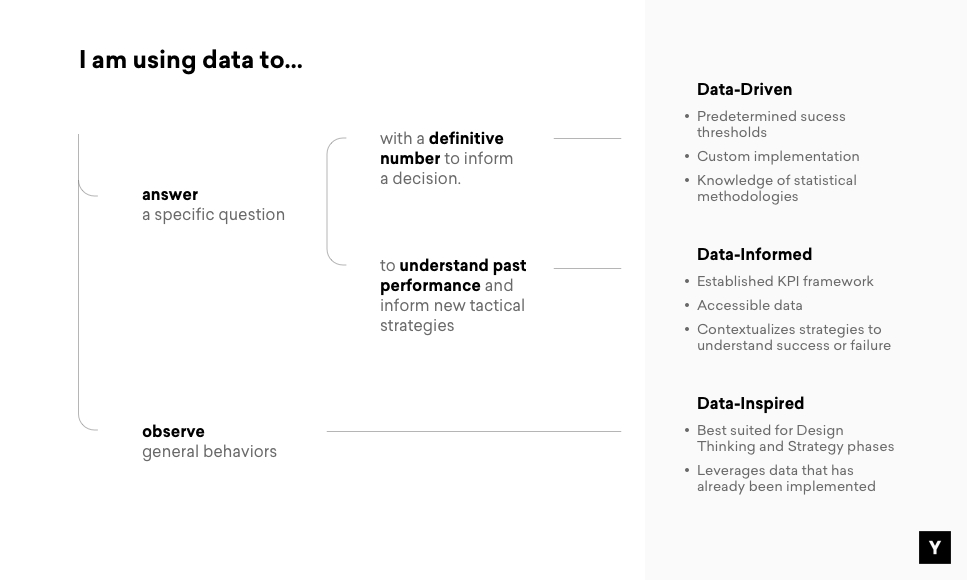
\includegraphics[width=15cm]{images/data-informed-graphic-ymedia-labs.png}
    \caption{I am using data to... (from Y Media Labs)~\cite{amplitude_are_you_data_driven}}
    \label{fig:i_am_using_data_to}
\end{figure}
%First discovered via \url{https://twitter.com/iteratively/status/1243641701408935936?s=20}

% SHOULD-DO write about: Identifying and designing data....

In a short paper~\citep{kidwell2015_toward_fault_taxonomy_application_of_software_analytics}, the authors propose combining fault classification and software analytics for five types of decisions. These are: targetting testing, release planning, judging stability, targeting training, and targeting inspection of software. failure data mined from software analytics tools such as crash reporting tools helps to bring their concepts and ideas to life. Their paper provided initial indicative evidence of their proposals through evaluation of changes to source code for the Eclipse software and discusses the measurement of refactoring to provide more accurate and relevant measurements of the efficacy of the refactoring, rather than considering approaches to improve mobile apps.


\subsection{Privacy and Control}

UW blog post~\cite{mcquate_I_saw_you_were_online} and the underlying CHI 2020 paper~\cite{cobb2020_ux_s_with_online_status_indicators} regarding how online status indicators shape their behaviour and on whether people know and can correctly control whether their data is being shared. Conversely, in his PhD thesis~\citep{adam2009balancing}, Adam noted that users of mobile devices were willing to withhold sensitive data provided they would not be found out. The users want blameless ways to control their privacy.

Mobile analytics collects a time-series of data online. In 2015, research into privacy concerns of continual observation identified a number of concerns with the erosion of privacy for users in these circumstances~\citep{erdogdu2015_privacy_utility_tradeoff_under_continual_observation}. The authors discussed various end-user concerns in having to trust the collection of their user data, including two trust boundaries: either locally, where~\emph{``the user may not entirely trust the aggregating entity in the first place,"} or at the aggregator's side - where the user trusts the entity collecting the data but not third-parties who may also gain access to the data. Either or both of these concerns may apply when users use mobile apps that collect analytics data. Their experiment that assessed whether six households could keep private their use of a microwave while simultaneously sharing data that enabled their washer-drier usage to be accurately tracked. Given the small-scale nature of the experiment it would be premature to determine whether the framework proposed in the research would also apply to mobile analytics, nonetheless the research offers a possible approach to increasing the privacy of mobile analytics data provided the data is still efficacious and sufficiently accurate for diagnostics, problem analysis, and reporting purposes.  % c.f. research into whether decentralised or centralised approaches are better for covid-19 tracking. See Without a trace: Why did corona apps fail? in the excluded works bibliography.

% Further reading
% https://www.kaggle.com/dansbecker/what-is-log-loss (refreshingly clear and succinct, I still don't quite understand the topic yet though...)
% A great title, I wish I understood the topic: "From the Information Bottleneck to the Privacy Funnel". Also their approach is unlikely to be used in mobile analytics software as there's little perceived practical need to provide privacy of this form :( 

% The purpose driven privacy preservation for accelerometer-based activity recognition 
The tradeoff between privacy and utility for data that can uniquely identify over 99\% of users from high-frequency data collection from accelerometers in mobile phones~\citep{menasria2018_purpose_driven_privacy_preservation_accelerometers}. Accelerometer data is one class of data that could be collected using mobile analytics. The paper discusses the compression of data that is disclosed so irrelevant private information can be reduced while also maintaining adequate utility of the analysis of the data that is disclosed. Their approach might offer the potential to reduce irrelevant private information collected by mobile analytics.

Privacy related violations by platform providers, including Apple and Google, where a user's phone (and presumably similar devices including tablet computers) are tracking users without the user's informed consent. A recent complaint was filed by NOYB - European Center for Digital Rights~\citep{noyb2020_noyb_files_complaint_against_apples_tracking_code_idfa} and reported by the Financial Times~\citep{ft2020_apple_tracks_iphone_users_without_consent}. The complaint is that iPhones track users and Apple shares the data with all the app developers. According to the article in the Financial Times, in June 2020 Apple promised their latest operating system, iOS14, would include a privacy dashboard and that apps would need to ask users for permission before accessing the unique IDFA (Identifier for Advertisers). However, again in this article~\emph{``Apple then said in September that it would delay the changes, “to give developers the time they need” until “early next year”."}. 



c.f. using infra-red cameras to detect people in ways they're unfamiliar with and do not expect. 

\section{Software Development Practices}

Topics include: Agile development and the effects of the software that's developed and released. Motivations for/of software developers.

\subsection{Papers to consider on software development practices}
\begin{itemize}
    \item \emph{A systematic review of theory use in studies investigating the motivations of software engineers}~\citep{hall2009systematic}.
    \item \emph{Designing Engineering Onboarding for 60+ Nationalities}~\citep{harty2020_designing_engineering_onboarding}. Onboarding software developers and staff generally also includes exceptions and exception handling. These exceptions can be collected and analysed to determine where the onboarding is failing. Again there can be the concept of non-fatal and fatal exceptions. Fatal exceptions shouldn't happen ideally, there are mechanisms to handle them adequately in terms of error recovery, however we'd like to know about them and address them.
    \item \emph{Enabling Productive Software Development by Improving Information Flow}~\citep{murphy_enabling_2019}. 
    \begin{itemize}
        \item ``The flow of information among software developers is directly related to productivity."
        \item ``When the flow of information is adequately supported, delivery times on software can be shortened, and productivity within an organization can rise."
    \end{itemize}
    \item \emph{Continuous delivery sounds great, but will it work here?}~\citep{humble2018_continuous_delivery_sounds_great}. 
    \begin{itemize}
        \item ``Continuous delivery is about reducing the risk and transaction cost of taking changes from version control to production. Achieving this goal means implementing a series of patterns and practices that enable developers to create fast feedback loops and work in small batches. This, in turn, increases the quality of products, allows developers to react more rapidly to incidents and changing requirements and, in turn, build more stable and higher-quality products and services at lower costs."
        \item ``If this sounds too good to be true, bear in mind: continuous delivery is not magic. It's about continuous, daily improvement at all levels of the organization—the constant discipline of pursuing higher performance. As presented in this article, however, these ideas can be implemented in any domain; this requires thoroughgoing, disciplined, and ongoing work at all levels of the organization. Particularly hard, though essential, are the cultural and architectural changes required."
    \end{itemize}
    
\end{itemize}


\section{Software Testing}

\subsection{Papers to consider}
\begin{itemize}
    \item TBC
    \item \emph{``Debugging without testing"}~\cite{ghardallou2016debugging_without_testing} It may be possible to demonstrate a bug has been fixed without testing, for instance by comparing behaviours before and after changes were made to the software. This paper's premise of being able to debug without testing held true in some of my research. Testing has not able to reproduce all the conditions needed for some bugs to emerge. Other information, such as stack traces, may help developers perceive likely causes of a bug, such as a crash, sufficiently for the developers to take what they believe is corrective action.  
    
    \item ~\emph{`Communication in Testing: Improvements for Testing Management'}~\citep{paakkonen2009_communication_in_testing}: 
    \begin{itemize}
        \item Three quality approaches: mapping of process, product, and quality-in-use => three perspectives: software engineer (developer), testing, and end-user. The first two are easier to measure for a software company, yet the quality-in-use is the most important for any product. \textbf{TBC}
    \end{itemize}
    
    \item Behaviourally Adequate Software Testing \url{https://leicester.figshare.com/articles/Behaviourally_Adequate_Software_Testing/10106189} - Behavioural Coverage, search-based white-box generation strategies. Measures of testing adequacy. \emph{One intuitive notion of adequacy, which has been discussed in theoretical terms over the past three decades, is the idea of behavioural coverage; if it is possible to infer an accurate model of a system from its test executions, then the test set must be adequate.} IIRC the programs they assess are tiny, and how can we determine 'accurate model', perhaps it'll be accurate for what it tests, but incomplete? "The truth, \emph{the whole truth}, and nothing but the truth" springs to mind. % See also Uncertainty-Driven Black-Box Test Data Generation (seems less relevant to my research) and Assessing Test Adequacy for Black-Box Systems Without Specifications (perhaps more relevant).
    
    \item Various papers listed on \url{https://testroots.org/publications.html} which focus on IDE measurements of developers running automated tests, CI and tests~\emph{``Oops, My Tests Broke the Build: An Explorative Analysis of Travis CI with GitHub"}, and code quality correlations between test and system code.
    
    \item "Probably approximately correct learning" however it seems to be unrealistic and impractical for shipping mobile app development teams.
\end{itemize}


\subsection{Concepts to consider}
\begin{itemize}
    \item Adequacy
    \item Confidence levels (in the testing we've done)
    \item Sufficiency (c.f. how Google graded OKRs where 0.7 was the expected, sufficient, amount of progress).
    \item What testing actually gets done for real software, rather than what testing standards, academia, etc. tells us we \emph{should} do.
    \item Probably Approximately Correct.
    \item Testing logging and analytics, especially when many aspects of the systems are provided by third-parties, involves determining causal links between two phenomena. Concommitant variations, introduced in~\cite{mill1884system}
    \item Who tests the software developers use? for instance the many APIs and libraries? Flaws in this software, created by others, may affect the development teams and the users of their software products, amongst others. This software will include proprietary code and will probably include opensource code, perhaps pre-packaged as libraries of binary code. Some of that software may be poorly maintained, and yet the quality of that software may adversely affect the quality of the code using it. 
\end{itemize}

\section{App Stores and their Effects on Software Development and Engineering}
The concept of an App Store has existed since at least 2003, according to the co-founder and CEO of Salesforce~\cite{benioff_trailblazer_2019}, where the idea was proposed by Steve Jobs and later implemented as \href{https://appexchange.salesforce.com/}{\emph{AppExchange}} in the Salesforce platform. Around the same period various app stores emerged for mobile apps~\footnote{Tens of app distribution platforms are listed on Wikipedia:~\href{https://en.wikipedia.org/wiki/List_of_mobile_app_distribution_platforms}{List\_of\_mobile\_app\_distribution\_platforms}}; and the concept seems to have been introduced around 1999 by Handandgo~\footnote{\url{https://en.wikipedia.org/wiki/Handango}}. Academic research into the effects of app stores emerged in or around 2010, for instance with the work of Kimbler who investigated the effects on mobile operators from a business strategy perspective~\cite{kimbler_app_store_strategies_2010} (who lost out in the overall battle of app stores, now platform specific app stores dominate the market). 

Also in 2010, early papers were published on various effects of app stores on academic research e.g. how app stores addressed some of the previous constraints such as reaching more users and facilitating the distribution of the apps and feedback from those users~\cite{cramer2010_research_in_the_large_app_stores, miluzzo2010research_in_the_app_store_era}. 

\begin{itemize}
    \item Cramer \emph{et al} discussed aspects of \emph{research in the large} and in particular for my research the importance of ``playing by the rules"~\cite{cramer2010_research_in_the_large_app_stores}. My research was also shaped to play by the rules of the app store.

    \item Miluzzo \emph{et al} introduced other relevant research aspects, \textit{i.e.}  ongoing concerns such as how to assess correctness when there is no \emph{``ground truth"} - a challenge when evaluating mobile analytics for shipping apps; and a software development model of \textit{``deploy-use-refine"}~\cite{miluzzo2010research_in_the_app_store_era}, where app development refines the app based on data gleaned from usage of the app. Our case studies used usage data to refine the app to improve the measured reliability of the apps. Their paper even explained how a silly mistake caused their app to crash where the app store then delayed the new release of the app by several weeks. Even in 2010 crashes adversely affected the app store's perception of an app. % Their work on CenseMe received an ACM Test of Time award, see https://www.cs.dartmouth.edu/~campbell/page-3/
\end{itemize}

\subsection{Papers to consider}
\begin{itemize}
    \item \emph{``App store effects on software engineering practices"}~\citep{alsubaihin2019app_store_effects_on_software_engineering}. \emph{``While automatic in-app crash reporting is the most prolific channel of reporting bugs, the one mostly prioritised by our respondents is user reviews in app stores."} - what are the effects of the crashes being a lower priority than user reviews? They don't discuss other sources of crash reports (e.g. platform crash reporting).
    
    \item \emph{``A survey of app store analysis for software engineering"}~\cite{martin2016survey, martin2017_survey_in_app_store_analysis_for_software_engineering_IEEE_edition}.
    
    \item \emph{``Why people hate your app: Making sense of user feedback in a mobile app store"}~\cite{fu2013people}. A key paper, many citations (some also highly relevant).
    
    \item \emph{``Analyzing and Automatically Labelling The Types of User Issues that are Raised in Mobile App Reviews"}~\cite{mcilroy2016analyzing} - discusses crashes, crash libraries, analytics, relatively early paper on the topic.
    
    \item \emph{``Revisiting the Mobile Software Ecosystems Literature"}~\cite{steglich2019revisiting} Helps to define what an ecosystem is.
    
    \item \emph{``Beyond Google Play: A large-scale comparative study of Chinese Android app markets"}~\cite{wang2018_beyond_google_play}.
    
    \item \emph{``Measurement, modeling, and analysis of the mobile app ecosystem"}~\cite{petsas2017measurement}.
    
    \item \emph{``A Measurement-based Study on Application Popularity in Android and iOS App Stores"}~\cite{liu2015measurement}.
    
    \item \emph{``Understanding the Evolution of Mobile App Ecosystems: A Longitudinal Measurement Study of Google Play"}~\cite{wang2019understanding} (2019): Lots of interesting questions and observations about Google Play; but they don't seem to consider flaws, or the effects of flaws, in the app store's data collection, algorithms, etc.
    
    \item \emph{``Release Practices for Mobile Apps--What do Users and Developers Think?"}~\cite{nayebi2016release}.
    
    \item \emph{``Towards Release Strategy Optimization for Apps in Google Play"}~\citep{shen2017_towards_release_strategy_optimization_for_apps_in_google_play}. ``empirical study to help developers decide the release opportunity to maximize positive feedback from users at scale.". They identify three patterns of update intervals: successive, normal, sparse. Their work does not use signals such as the stability of the app. They also claim ``Additionally, app quality can be unstable with fast [release] iteration[s]."
    
    \item \emph{``Determinants of Mobile Apps' Success: Evidence from the App Store Market"}~\citep{lee2014_determinants_of_mobile_app_success_evidence_from_the_app_store_market} Survivorship for apps, hazard models, quality updates one of the topics in the paper. iOS - Apple App Store. A focus on sellers rather than app developers. Figure 1, sustainability of app sales: empirical approach. 4 Hazard models App Quality update (App\_quality\_update): \emph{``1 if an app’s quality indicators were updated (adding more app features or fixing bugs)"}. Survivorship in the app store ecosystems and what devs can do to increase their app's survival. Seller [app developer]-level decisions, app-level decisions, user response to the decisions. It doesn't discuss app store algorithms or their effects. c.f. the more recent articles on iTunes rankings of apps from Medium.com~\citep{lotan2015_apple_apps_and_algorithmic_glitches, lotan2015_apples_app_charts}.
    
    \item \emph{``Feature lifecycles as they spread, migrate, remain, and die in App Stores"}~\cite{sarro2015_feature_lifecycles_in_appstores} discusses \emph{adaptive development} as a concept for developers of apps in app stores. Notes: Their research is based on `non-free features from two app stores (Samsung and Blackberry)' (both relatively dwarfed by Google Play) and their work predates the availability of platform level analytics, etc. Relevance to my work: developers can obtain requirements (in terms of work they're potentially `required' to do) from many sources, including direct feedback from end users of the apps, signals in terms of willingness to install and keep using their app, and from analytics. Developers want and increase the value of their work by prioritising potential work appropriately. Signals and data from mobile analytics may provide useful, additional sources of information that's sufficiently relevant for developers to accept these `requirements' and address them.
    
    \item \emph{``Which version should be released to app store?"}~\cite{nayebi2017version}.
    
    \item \emph{``Modern release engineering in a nutshell - why researchers should care"}~\cite{adams2016modern}.
    
    \item The \emph{``Data analytics for decision support in software release management"}~\cite{didar2018data_analytics_phd_thesis}, a PhD thesis, introduces a proposed Plan-Monitor-Improve Framework for release management.
    
    \item \emph{"An Explorative Study of the Mobile App Ecosystem from App Developers' Perspective"}~\cite{wang2017_exploratory_study_of_the_mobile_app_ecosystem}: 1,000,000+ apps on Google Play, 320,000 developers, over half of the developers only released a single app. The paper mainly focuses on the \emph{"the group of aggressive developers who have released more than 50 apps, trying to understand how and why they create so many apps"}. Provides some context on who writes the mobile apps in Google Play, provides an estimate of the population of developers (in 2017).
    
    \item \emph{``Requirements Intelligence: On the Analysis of User Feedback"}~\cite{stanik2020requirements_intelligence_on_the_analysis_of_user_feedback}. continuous sources for requirements-related information; comparison between explicit and implicit user feedback (like app usage data).
    
    \item \emph{``Are apps ready for new Android releases?"}~\cite{guilardi_are_apps_ready_for_new_android_releases}. A current (2020) paper where the researchers discovered that developers are slow to revise and update their Android apps for new releases of the operating system. Some of the apps have flaws exposed when running on new versions of the operating system. For apps to retain their quality they need to be updated, new releases of the operating system are one such reason. (Releases of libraries another, new contexts of use, etc. another...).
    
    \item \emph{``Revisiting Prior Empirical Findings For Mobile Apps: An Empirical Case Study on the 15 Most Popular Open-Source Android Apps"}~\citep{syer2013_empirical_findings_for_mobile_apps} is work from 2013 (when Google Code was still a major active public source code repository) that compares the codebases of 15 opensource mobile apps with 5 other opensource desktop/server projects. A key finding in their research includes the development process - where there are frequent releases yet the development and release processes are immature. albeit based on codebases from 2011 so a decade ago is still relevant. They ask various open-ended questions:
    \begin{itemize}
        \item Does such a high frequency of releases mitigate the lack of testing? 
        \item If there are frequent releases for the mobile app, then does quality matter as much?
        \item Is the project in a constant beta testing state? 
        \item Does the platform provide sufficient support for building high quality apps quickly? 
        \item Is the frequent release only influenced by the demand factor in the app store? 
        \item Are the developers of mobile apps more skilled or do they have more resources at hand? 
        \item Or, are mobile apps themselves less complex to develop?
    \end{itemize}
    
    Perhaps the cost of failures in the app store was/is perceived to be low in the Google Play app store, at least for these 15 opensource apps? Later work investigated aspects such as the release frequency~\citep{nayebi2016release}
    
    \item Both Medium articles by Gilad Lotan in 2015 on Apple's App Store rankings provide intersting colour to the discussion of the rankings over time~\citep{lotan2015_apple_apps_and_algorithmic_glitches, lotan2015_apples_app_charts}; however they're not directly relevant to software development practices so might not be that relevant.
    
\end{itemize}


App Stores behave as intermediaries between developers and the users of their software. They make various aspects more transparent including pricing, information about the apps, releases, and ratings \& reviews. There are hundreds of thousands of developers of Android apps according to various sources (320,000 in 2017~\cite{wang2017_exploratory_study_of_the_mobile_app_ecosystem}, ...).


In an App Store first the developer then the app store are involved in making a release available to some or all of the user population. There are various competing factors that affect when would be a good time to make a release. Too few and an app may be considered stale or neglected, too many and users may balk at the seemingly endless updates and communications costs. Groups of researchers have investigated various aspects of release engineering, including~\cite{adams2016modern} that argues the relevance of modern release engineering and the relevance for researchers, and~\cite{nayebi2017version} which concentrates on which version of opensource apps should have been released to the app store. Developers, and their stakeholders, want to make more informed decisions about which releases to make; however there does not appear to have been much research into the testing and quality indicators available to app developers before they make their release public.


\section{Developing Mobile Apps}

\subsection{Papers to consider}
\begin{itemize}
    \item TBC
    \item \textbf{Species of Bugs}
    \item J2ME write once debug on a million devices quote?
    \begin{itemize}
        \item \emph{``Finding resume and restart errors in Android applications"}~\cite{shan2016finding}. Which leads to "Large-scale analysis of framework-specific exceptions in Android apps" (2018) where the exceptions should be detectable by Android Vitals, I hope.
        \item \emph{``JInjector"} the makeup of mobile apps~\citep{sama2009using_jinjector}. \emph{``Statistically most of the code in a J2ME application belongs to the GUI;"}. The tool was also applied to Android apps and provided similar capabilities to instrument the GUI. Null Pointer Exceptions (which affect both Android Java apps and J2ME apps) can elude the development and testing pre-release of apps, even from Google-calibre software engineers. Freezing in J2ME apps were also detected, and freezing is one of the factors measured by the Android platform and reported as ANRs.
        \item \emph{Do android developers neglect error handling? a maintenance-centric study on the relationship between android abstractions and uncaught exceptions}~\citep{Oliveira_Borges_Silva_Cacho_Castor_2018_android_error_handling}.
    \end{itemize}
\end{itemize}




\subsection{Bugs}
Species of bugs: inadequate and neglected error handling, data loss bugs.

Exception handling is strongly related to program robustness.~\citep{Oliveira_Borges_Silva_Cacho_Castor_2018_android_error_handling}. In particular, they observed that developers did not write sufficient code to handle exceptions that could be thrown when their Android app uses Android-specific abstractions. Uncaught exceptions lead to the application crashing, and crashes are an indication of poor reliability of the application. Of course, the exception needs to occur in order for the app to crash, and not every uncaught exception causes the app to crash, they may crash an internal thread within the app instead~\citep{Oliveira_Borges_Silva_Cacho_Castor_2018_android_error_handling}. %Note: not all caught exceptions are handled adequately. E.g. some may simply be logged and the code allowed to continue unchanged. Sometimes the exception may mean internal state and/or data are incomplete or incorrect for reliable and correct operations of the app. 
Their research excluded various factors that also affect robustness, in particular they chose not to study: ``security vulnerabilities, excessive resource consumption, and race conditions."~\citep{Oliveira_Borges_Silva_Cacho_Castor_2018_android_error_handling}. %As an observation, they appear to over-state the LOC they analysed, or at least they're inflating the counts to count every line of code six-times even if those lines are identical for two or more releases.

In the work of~\citep{khalid2015_what_do_mobile_app_users_complain_about} the authors note that iOS apps with frequent functional errors or crashes are more likely to be rated poorly in the app store. Their work did not extend to Android apps, however it seems reasonable that errors and crashes in Android apps would also lead to lower ratings in the app store, and conversely Google states that~\emph{``Performance and stability are directly linked to positive ratings on Google Play."}~\citep{android_vitals_best_practices}.

\textbf{MUST-DO} write about the fault-proneness paper reference on Android APIs~\citep{linares2013_api_change_and_fault_proneness_android}.
% via Oliveria... 
% Linares-Vásquez et al. (2013) investigated the relation between the success of Android applications (in terms of user ratings) and the change- and fault-proneness of the underlying APIs. They have computed bug fixes and changes in the interfaces, implementation and exception handling of 7.097 Android applications belonging to different domains. They found that APIs used by successful apps (high user ratings) are significantly less change- and fault-proneness than APIs used by unsuccessful apps. In terms of changes to the set of exceptions thrown by methods, the study did not observe any significant difference between different levels of rating.

% via Oliveria...
% Bhattacharya et al. (2013) performed an in-depth empirical study on bugs in 24 widely-used open-source Android apps from diverse categories such as communication, tools, and media. They sought to understand the nature of bugs and bug-fixing processes associated with smartphone platforms and apps. They defined several metrics to analyze the bug fixing process. They showed how differences in bug life-cycles can affect the bug fixing process and performed a study of Android security bugs. 

\emph{``Characterizing Android-Specific Crash Bugs"}~\citep{jha2019_characterizing_android_specific_crash_bugs} TBC.


Data loss bugs: When apps lose data they also lose the trust of users. One cause of data loss in Android apps has been investigated recently (2019) in ~\cite{riganelli2019benchmark_android_data_loss_bugs} where the authors found 19.2\% of the Android apps they evaluated lost data. The data losses were of one particular type - where the app failed to save and/or restore data when the app was stopped and restarted. There are other causes of data loss for mobile apps including database, network and storage errors, for example. They claim some of these bugs may surface as crashes in the app at a later stage, after the data was lost and the app resumed, however their examples did not seem to result in crashes. \yijun{Data loss is definitely a sign of lack of integrity. Sometimes it is required to lose some user data for privacy protection. Maybe you can refine the definitely more precisely to refer to "retaining the data that users care".} \yijun{I think one of the gaps is that the data loss bug that does not lead to crashes are actually bugs too. This is kind of important to justify your work will be different from other app testing literature that focus on detecting crash related bugs.}

To the authors' credit they provide extensive material including automated tests for the vast majority of the bugs~\footnote{\url{https://gitlab.com/learnERC/DataLossRepository}}. They were able to create automated tests that reproduced 110 of the 116 errors and were able to automatically detect 98 out of the 110 errors they were able to reproduce.

One of the considerations this work helps to illustrate is the many challenges of measuring software quality comprehensively, or even adequately.

\textbf{TODO} Wrap up this sub-section with where most of the research has been in terms of bugs in mobile apps.

\hypertarget{mobile.testing}{}
\section{Testing Mobile Apps}

\subsection{Papers to consider}
\begin{itemize}
    \item \emph{``To the attention of mobile software developers: guess what, test your app!"}~\citep{cruz2019_guess_what_test_your_app}.
    
    \item \emph{``PRADA: Prioritizing Android Devices for Apps by Mining Large-Scale Usage Data"}~\citep{lu2016_PRADA}. 
        
    \item \emph{``Automatically Discovering, Reporting and Reproducing Android Application Crashes"}~\citep{moran2016_automatically_drr_android_app_crashes}.
    
    \item \emph{``Is Mutation Analysis Effective at Testing Android Apps?"}~\citep{deng2017_is_mutation_analysis_effective_at_testing_android_apps}.
    
    \item \emph{``Mining Android Crash Fixes in the Absence of Issue- and Change-Tracking Systems"}~\citep{kong2019_mining_android_crash_fixes}.
    
    \item \emph{``How do Developers Test Android Applications?"}~\citep{linares2017_how_do_developers_test_android_apps}. Quote:~\emph{``“I mostly do manual testing due to the limited size of my apps. I sometimes use a custom replay system (built into the app) to duplicate bugs after I come across them. This method is usually combined with manual testing (printing debug information to the log) to pinpoint the cause”."}
    
    \item \emph{``Prioritizing the Devices to Test Your App on: A Case Study of Android Game Apps"}~\citep{khalid2014_prioritizing_the_devices_to_test_your_app_on_casestudy_android_games}.
    
    \item \emph{``First Steps in Retrofitting a Versatile Software Testing Infrastructure to Android"}~\citep{oliver2018_first_steps_in_retrofitting_a_versatile_sw_testing_architecture}.
    
    \item \emph{``A Large-Scale Study of Application Incompatibilities in Android"}~\citep{cai2019_large_scale_study_of_android_incompatibilities} An oddly insipid paper which promised some interesting run-time issues discovered in their research where the Android version would be a likely cause. However the reproduction package lacked the test scripts or means to reproduce their testing or bug detection. Also, their research now seems to be less relevant in 2020 as Android apparently improved the backwards compatibility \emph{``Yet newer versions (since API 24) had no run-time compatibility issues with apps created in the studied span."}. Their work may well have merit for the research community, It does not appear to have much relevance to developers of real-world Android apps today.
    
    \item \emph{`A Case Study of Automating User Experience-Oriented Performance Testing on Smartphones"}~\citep{canfora2013_automating_UX_experience_testing_on_smartphones}. %30 citations in Google Scholar. 
    This research focused on whether their ATE (Automated Testing Equipment) could detect and score perceived UX of two versions of an Android phone, the HTC~\textsuperscript{\textregistered} Nexus One. The key difference was a reduction of RAM by 30\% which made their simple Android application slower on the version with less RAM. They used and processed Android logs to record the differences in timing information. Their ATE provided similar quality scores to human volunteers who used both versions of the phone. Their ATE equipment incorporated servo motors to move the phone around on an otherwise fixed testbed and a camera to record the GUI. (Curiously their photo shows they were using a Samsung phone rather than the one described in the paper.) The paper lacked details of the hardware, the movements the servos provided, or of the simple Android application they created and used for their evaluation.
    Note: Their approach in moving the phones appears similar to that used by LessPainful (a now defunct company, since acquired ultimately by Microsoft) who provided a commercial testing service across a wide range of Android \textit{and} iOS devices. 
    This paper's work is relevant for its use of Android logs and logging to record and analyse the usage of the device. Unfortunately there appear to be several material flaws in the paper, for example where they state: ~\emph{`...a score of 30 for CUST-37..."} the only mention of CUST-37 whereas the rest of the paper refers to a CUST-30 configuration (with 30\% less RAM). Have they transposed the two numbers ~\emph{e.g.} should it be a score of 37 for CUST-30? and on a related note, their calculation of the percentage difference in their ATE generated UX score says the CUST-30 received a score of 4.05/5 while the stock configuration received a score of 4.54/5. While the difference in the scores by the humans of 4.54/4.05 is approximately 12\% these scores are out of 5, so the percentage should be twice the one they used ~\emph{i.e. approximately 22.42\%}  \texttt{=((4.54/4.05)/5.00)*100\%}.
    
    \item \emph{``Intent Fuzzer: Crafting Intents of Death"}~\citep{10.1145/2632168.2632169} TODO Link this to the industrial case study and the Kotlin NPE crash.
    
    \item \emph{`A Grey-Box Approach for Automated GUI-Model Generation of Mobile Applications'}~\citep{Yang_Prasad_Xie_2013_grey_box_automated_gui_model_generation_for_mobile_apps}: This is one of the relatively early papers that focused on model-based testing for mobile apps. They used a simpilified version of a simple tip calculation app as their example application under test. They further similify the complexity by ignoring changes in the application state related to different data values. Their work built on the work of various approaches to `crawling' GUIs of an application and provides one of the roots of automated dynamic interactions with fairly simple opensource Android applications. It achieved good coverage for these apps. Through no fault of their research mobile apps, and particularly successful mobile apps are far removed from the apps they tested and their approach and tool has fallen into disuse. %Nonetheless two of the authors were granted a US patent for their approach in 2019! :( Automatically extracting a model for the behavior of a mobile application. MR Prasad, W Yang - US Patent 10,360,027, 2019
    
    \item "Mobile Testing-as-a-Service (MTaaS)--Infrastructures, Issues, Solutions and Needs"~\cite{gao2014mobile}. This paper, published in 2014, in my view isn't particularly novel. Rather it summed up stuff that was happening in industry at the time and combined it with a bunch of ideas of what \emph{might} be worth doing in the authors' view. The aim of the authors is to set the direction for scaling testing of mobile apps. Six years on is a good time to assess their suggestions.
    
    \item "The Testing Method Based on Image Analysis for Automated Detection of UI Defects Intended for Mobile Applications". \textbf{Springer paper I paid for.}
\end{itemize}

There has been a tremendous and sustained research interest in software testing, for instance testing is one of the most popular topics at the ICSE series of conferences~\footnote{\url{https://dl.acm.org/conference/icse}} and the focus of entire conferences including AST~\footnote{\url{https://conf.researchr.org/home/icse-2020/ast-2020}}, ICST~\footnote{\url{https://conf.researchr.org/series/icst}}, and so on. Similarly the application of software testing to mobile apps is a rich topic with sustained interest in the challenges and facets of testing mobile apps.

The facets include automated testing and automated bug reproduction, maximising the `bang for the buck' for instance in selecting which device models would be most valuable to use with finite testing. Understandably given the field where many of the authors work - in research - the vast majority of the research is on software apps they have access to, software their can obtain the source code for (particularly opensource), software they can write, and the people they have available to them (other researchers, students, voluntary participants, and people paid to paid to perform specific tasks). Minute amounts of the work is based on mature, popular software with semi- or fully- professional developers and development teams. Some research projects, particularly CRASHSCOPE~\citep{moran2016_automatically_drr_android_app_crashes}, offer the potential to reproduce some of the crashes reported by Mobile Analytics if the tools are sufficiently available and current to actually use.



There is some interesting large-scale research into analysis of various releases of production Android application binaries~\citep{kong2019_mining_android_crash_fixes}. The researchers exercised (tested) a large range of apps seeking crashes of the app using an oracle of a local log file which they queried using the standard Android \texttt{logcat} utility. They also combined their dynamic approach with using static analysis tools to identify potential flaws that would lead to crashes of an app. They then tested newer releases of the same app. If the newer version did not crash they analysed the binary files (the APK files) for both releases to differences to the compiled code that may have been responsible for 'fixing' the crash. They limited their work to Android \emph{framework specific} crashes, and excluded \emph{app-specific} crashes. They devised ways to identify changes that appeared to fix the particular crash(es) they triggered in the earlier releases and generated patch files based on these changes. These patches were then applied to the older release of the app and the app then tested with the same test inputs and runtime environment (at least in terms of using a consistent Android Emulator (also known as a virtual device)). They provide a relatively detailed replication package online at~\url{https://craftdroid.github.io/}.

\begin{itemize}
    \item Their approach is innovative and could help real-world developers of Android apps to identify and apply snippets of code to reduce the likelihood of their app suffering the same crash. Their 17~\href{https://github.com/CraftDroid/ExpData/tree/master/Fix_Templates}{fix templates} act as guides for Android developers and could potentially be implemented into code-quality tools.
    \item However it only applied for framework specific crashes, and their choice of runtime environment meant they could only install 56\% of the APKs. There are many other sources of crashes, and also apps that include native code (several of my case study apps do). Also their testing is limited to automated `monkey' testing which may further limit the crashes their approach can find in production apps, particularly those that incorporate user accounts, user-specific content, behaviour, online purchases and many other forms of activities.
    \item The supporting website \url{https://github.com/CraftDroid} includes scripts and log extracts for the crash reproductions, it lacks the mechanisms for generating diffs, applying them, or building the patched APK. The lack of these mechanisms makes the efficacy of their approach hard to reproduce.
    \item It also does not appear to test for crashes related to third-party libraries e.g. OkHttp which is extremely popular in Android apps; however potentially this approach could be extended to do so?
\end{itemize}

In summary, the approach proposed in~\citep{kong2019_mining_android_crash_fixes} has the potential to mine crash stack traces (which are available to the developers of the particular apps) to help with aspects of reproducing a subset of those crashes which pertain to Android framework-related crashes. Similarly it appears it could complement the automated testing provided by Google as part of the pre-launch reports available in Google Play Console and other services. 

\subsection{Prioritising devices to test on}

Selection criteria include:
\begin{itemize}
    \item the relative popularity of a single app across the user base for the app, provided by OpenSignal, and reported over a three year period,
    \item the usage of similar, popular, Android apps for two app categories: grouped by device model as measured by a very popular app management app in China,
    \item the devices used most frequently by users who write reviews for the same Android app,
\end{itemize}

One of the research papers close to the area of my research uses usage data for two popular app categories (games and media) gathered through a popular Android management app in China~\citep{lu2016_PRADA}. Their work uses an operational profile to prioritise the device models to select to test both new or existing apps. The management app, called Wandoujia~\footnote{\url{https://www.wandoujia.com/}}, is used by \emph{`500 million people to find apps they want`}~\footnote{According to Chrome Browser's automatic translation from Chinese.}. Daily usage of the top 100 apps in the two app categories was collected for various device models. In various ways the Wandoujia app management app provides similar capabilities to Google Play, including tracking when apps are installed, and in use. The recommendations are coarse-grained. The research measured the accuracy of their predictions for recommended devices with the actual devices that the app ended up being used on once the app had been launched. 

Their work demonstrates that usage data for several app categories was useful to guide developers on the most popular actual device models for their app. They acknowledge several limitations in their work, including their use of incomplete measures such as foreground network activity for usage which don't suit apps that either perform network processing in the background or don't use the network. Other app management services, particularly Google Play, could provide similar guidance to app developers. And indeed as Google Play collects additional data for the entire apps store it could cover some of the gaps and limitations identified in this research.


\hypertarget{mobile.analytics}{}
\section{Mobile Analytics}
\label{rw-mobile-analytics-papers}
\subsection{Papers to consider}
\begin{itemize}
    \item \emph{``"}~\citep{parate2016_RECKON_an_analytics_framework_for_app_developers_HP_AppPulseMobile} describes how automatic instrumentation of mobile apps using mobile analytics tools including HP's App Pulse Mobile is able to help developers better understand their users. 
    \item \emph{```Bad Smells" in software analytics papers'}~\citep{menzies2019_badsmells_in_software_analytics}.
    \item \emph{Software analytics for mobile applications--insights \& lessons learned}~\citep{minelli2013_software_analytics_samoa}. Their online site is still up \url{http://samoa.inf.usi.ch/}
    \item \emph{``Mining Device-Specific Apps Usage Patterns from Large-Scale Android Users"}~\citep{li2017_mining_device_Specific_app_usage_patterns}
\end{itemize}

Direct vs indirect analytics - 
Challenges of research into usage-derived analytics - perhaps why there are gaps in knowledge, compounded for indirect analytics. A tale of two apps, any others?

\subsubsection{Device Testing Services}
Test Farms have been available commercially since around 2008~\footnote{Based on the author's professional experience.}. Over the years different offerings have peaked and then either been acquired, retired, or disappeared. Google, Amazon and Microsoft offer paid-for device farms as do various specialist businesses. There have been a couple of public-good initiatives including Open Device Labs~\footnote{For example~\url{https://opendevicelab.com/},~\url{https://www.devicelab.org/}}; and Open STF~\cite{openstf_website} which is based on a set of opensource projects~\url{https://github.com/openstf/} and enables teams and organisations to build their own device farms or use commercial offerings based on these projects~\footnote{For example~\url{https://www.headspin.io/}.}.
% https://loadfocus.com/blog/tech/2018/04/building-your-in-house-device-farm-on-mac-os-using-openstf-for-android-testing/ 
% https://tech.mercari.com/entry/2019/02/18/173236 (on using HeadSpin and NimbleDroid).



\section{Placeholder for related work migrated from elsewhere in this thesis}
There are several key survey papers, the following was written in the RQ section as part of determining that this research is a) relevant and b) hasn't been covered by others. The contents need to be woven into the rest of the thesis.

\begin{mdframed}[style=MyFrame]
\emph{Future Trends in Software Engineering Research for Mobile Apps}~\citep{nagappan2016_future_trends_in_sw_eng_for_mobile_apps} focuses attention on the software development life-cycle, as illustrated in Figure~\ref{fig:nagappan2016_future_trends_in_sw_eng_for_mobile_apps_figure_1_annotated}, it does not investigate usage or operational aspects.

    {\centering
    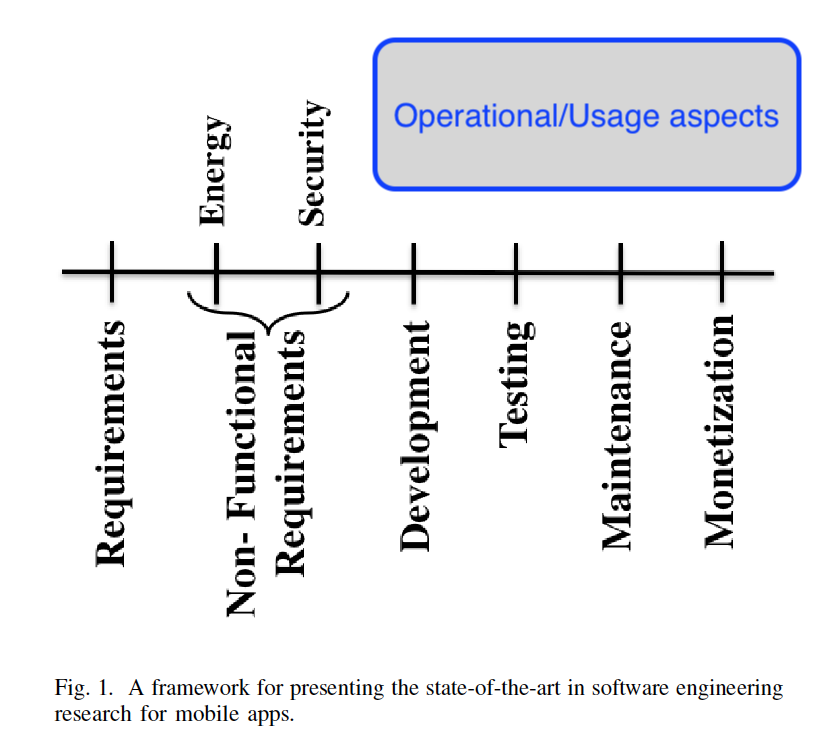
\includegraphics[width=11cm]{images/related-work/future-trends-in-sweng-for-mobile-apps-fig-1-annotated.png}
    \captionof{figure}{Annotated version of the framework for presenting the state-of-the-art in software engineering for mobile apps SANER2016~\citep{nagappan2016_future_trends_in_sw_eng_for_mobile_apps}}
    \label{fig:nagappan2016_future_trends_in_sw_eng_for_mobile_apps_figure_1_annotated}
    } % Thanks to https://tex.stackexchange.com/a/232290/88466

Mining review data for various forms of data including requests for bug fixes as is using rating as an assessment of goodness. 
Figure~\ref{fig:nagappan2016_future_trends_in_sw_eng_for_mobile_apps_figure_2_annotated} is an annotated version of their `Figure 2'. Various sources of information can be used by the development team, of these ratings and reviews are broadly researched, whereas device-level and app-level analytics have not been previously researched.

    {\centering
    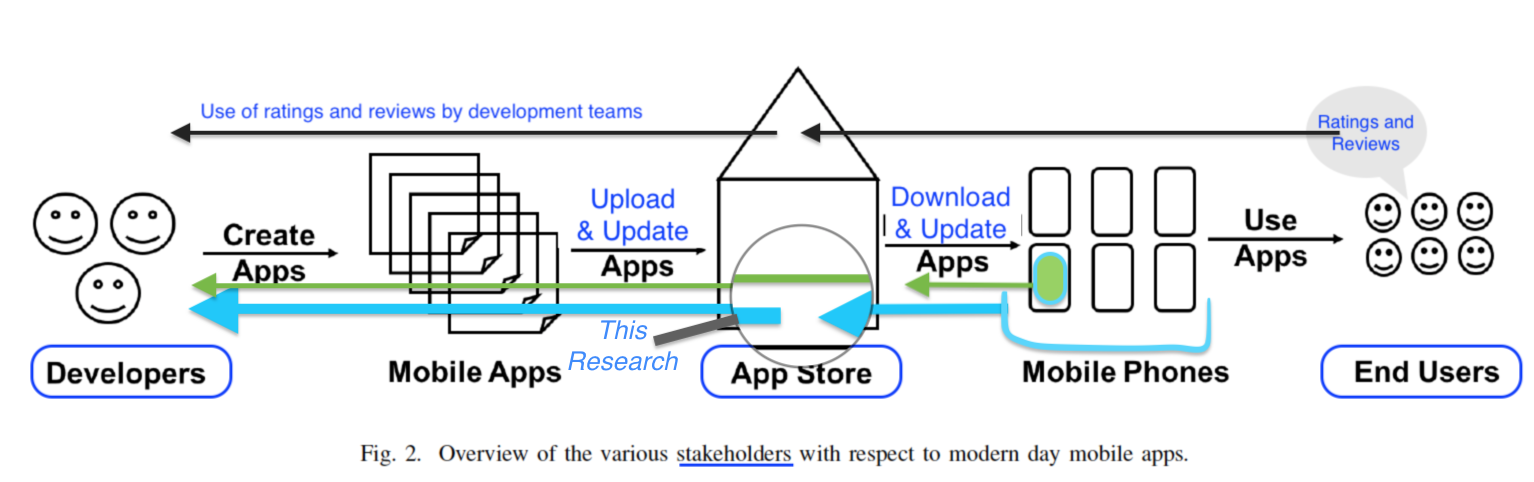
\includegraphics[width=12cm]{images/related-work/future-trends-in-sweng-for-mobile-apps-fig-2-annotated-with-highlights.png}
    \captionof{figure}{Annotated version of the various stakeholders in the modern app store ecosystemSANER2016~\citep{nagappan2016_future_trends_in_sw_eng_for_mobile_apps}}
    \label{fig:nagappan2016_future_trends_in_sw_eng_for_mobile_apps_figure_2_annotated}
    }

One of the key challenges identified is restricted access to data held by the app store, and that the only way to gather historical information is to continually mine the app store on a regular basis.

Are failure data potentially a form of requirements? (in a similar fashion to leveraging reviews in the app store to extract `requirements'). And similarly can complaints and failure data be combined to help developers prioritise issues they should consider addressing (the paper restricted the discussion to prioritising issues the developers should be \textit{testing} for).

The authors of the paper discuss limitations they experienced, perhaps without being aware that developers of Android apps have long term access to all the reviews of their apps. Details of how developers can download these and other reports, including the data structures, are available online~\citep{google_play_download_and_export_monthly_reports}. 

\emph{``Linares-Vasquez et al. [56] propose MonkeyLab, which mines recorded executions to guide the testing of Android mobile apps."} Their approach records GUI events (click events). Members of the project team (developers, testers, etc.) perform the actions, the authors claim their log collection process could scale to collecting logs from ordinary users. Key limitations include events that aren't purely dependent on the user's GUI inputs, there would also be challenges getting users to accept such an approach where the app records every input they made. Also, they generate GUI events that have x,y coordinates - absolute positioning that may have limited portability to other devices, screen rotations, and so on. Their playback also appears to require rooted devices. There are numerous other limitations described in their paper, nonetheless their work shows promise in terms of detecting and generating patterns the students did not find. It would be interesting to compare the results using accomplished software testers with experience and expertise testing similar Android apps.

Building on a point made in this paper: \emph{``the future of app quality engineering is data driven."}~\citep{maalej2016_towards_data_driven_requirements_engineering} % cite 97.

\emph{``Thus even if the app is tested on one device, there is no guarantee that it may work on another device."} - I agree. They don't provide any substance for this statement.

\emph{``The area of software maintenance is one of the most researched areas in Software Engineering. However, due to the fact that mobile apps is a young subarea within SE, the maintenance of mobile applications remains to be largely undiscovered."} - My work does investigate aspects of maintenance. 

\emph{``Syer et al. [93] compares mobile apps to larger “traditional” software systems in terms of size and time to fix defects. They find that mobile apps resemble Unix utilities, i.e., they tend to be small and developed by small groups. They also find that mobile apps tend to respond to reported defects quickly."} - Check the details of what quickly means and how the teams discovered the defects.

\emph{``Bavota et al. [16], show that the quality (in terms of change and fault-proneness) of the APIs used by Android apps negatively impacts their success, in terms of user ratings. Similarly, McDonnell et al. [65], study the stability and adoption rates for the APIs in the Android ecosystem."} - Skim read both these papers to determine their relevance.

\emph{``Another line of work examined Android-related bug reports. Bhattacharya et al. [18] study 24 mobile Android apps in order to understand the bug-fixing process. They find that mobile bug reports are of high quality, especially for security related bugs. Martie et al. [63] analyzed topics in the Android platform bugs in order to uncover the most debated topics over time. Similarly, Liu et al. [58] detected and characterized performance bugs among Android apps."} - Looks at how the bugs were fixed and compare the practices they detected with those I'm aware of. Are platform bugs that relevant? They look at performance bugs (Android Vitals also reports performance issues, Firebase Analytics has tools for performance tracking), I'm looking mainly into reliability measurements and issues.

Following on from the challenges and future directions section on maintenance research for mobile apps: do researchers focus in areas where the streetlights are rather than where the problems are? \emph{i.e.} on where they can find material to study rather than on issues that practically affect the majority of developers of apps?

\emph{``One interesting line of future research is in estimating the maintenance cost for a mobile app. Currently there are just anecdotal estimates [3]."} - Skim read this paper.

An opening gambit for my research: \emph{``Finally as mentioned in Section IX, there are several companies that collect operational data from mobile apps that have been installed on millions of devices. Most of these companies provide the app developers with the data and some rudimentary analysis on them. There is a wide variety of reliability and performance problems that can be solved by building tools and approaches that mine such operational data (past work has barely scratched the surface of such a problem by looking more at the server side of mobile applications than the client side [92])."}

Monetization is a post-release measurement, where revenues and other business-oriented metrics are applied to consider the successfulness of a mobile app. Although the paper focuses on small development teams (see the following quote as an example) in my experience many developers have measures they use in order to assess their prior work and focus their immediate future work. 
\emph{``In such apps where the development organization is small, often the developers will also have to make several engineering decisions that could affect their bottom line. Therefore software engineering researchers have examined how we can provide data to mobile app developers so that they can make these decisions in a more careful fashion."} This may be useful to support the bug triage process that developers use when determining which of the reliability bugs they choose to fix.

\emph{``Currently there are also several analytics companies (AppAnnie [1], Quettra [9], Crittercism [6] etc.) that provide valuable usage data to developers for improving their monetization strategies. They track the downloads of apps, and how the apps are being used, when users purchase things from the app etc. These companies are able to track such user data, by incorporating tracking libraries in the mobile devices. Using this information developers are able to make smarter data driven decisions with respect to making their app more successful. However, most of these recommendations are more from a marketing perspective than software engineering perspective."}
There's a lot to unpack here. Firstly although this topic discusses monetization strategies, the use of analytics can also help developers make smarter data driven decisions with respect to making their app more successful from a~\emph{software engineering} perspective. Secondly, the tracking libraries mentioned here are added to the app rather than to the device. 
\begin{itemize}
    \item AppAnnie~\citep{appannie2021}: 
    \item Crittercism: rebranded as Apteligent, which was acquired by VMWare in 2017. A few traces remain on StackOverflow and GitHub, etc. of Crittercism's analytics products of 2015. Essentially crash reporting. Some integration into enterprise systems e.g. to Splunk.
    \item Quettra: Acquired by SimilarWeb~\citep{techcrunch2015_quettra_mobile_analytics_acquired} their focus was described as a deep understanding of the users, which was then intended to help developers improve retention and also improve targeting of adverts.
\end{itemize}

\emph{``There has been some recent initial work in this direction where Bavota et al. [16] looked at the impact of using certain APIs on the ratings and Tian et al. [94] model a set of factors (like size of app, complexity of app and its UI, quality of the library code etc.) against the ratings. They were able to find that there is initial evidence that high rated apps have a certain DNA (certain value for various factors)."}

\end{mdframed}
